% Options for packages loaded elsewhere
\PassOptionsToPackage{unicode}{hyperref}
\PassOptionsToPackage{hyphens}{url}
%
\documentclass[
]{book}
\usepackage{lmodern}
\usepackage{amsmath}
\usepackage{ifxetex,ifluatex}
\ifnum 0\ifxetex 1\fi\ifluatex 1\fi=0 % if pdftex
  \usepackage[T1]{fontenc}
  \usepackage[utf8]{inputenc}
  \usepackage{textcomp} % provide euro and other symbols
  \usepackage{amssymb}
\else % if luatex or xetex
  \usepackage{unicode-math}
  \defaultfontfeatures{Scale=MatchLowercase}
  \defaultfontfeatures[\rmfamily]{Ligatures=TeX,Scale=1}
\fi
% Use upquote if available, for straight quotes in verbatim environments
\IfFileExists{upquote.sty}{\usepackage{upquote}}{}
\IfFileExists{microtype.sty}{% use microtype if available
  \usepackage[]{microtype}
  \UseMicrotypeSet[protrusion]{basicmath} % disable protrusion for tt fonts
}{}
\makeatletter
\@ifundefined{KOMAClassName}{% if non-KOMA class
  \IfFileExists{parskip.sty}{%
    \usepackage{parskip}
  }{% else
    \setlength{\parindent}{0pt}
    \setlength{\parskip}{6pt plus 2pt minus 1pt}}
}{% if KOMA class
  \KOMAoptions{parskip=half}}
\makeatother
\usepackage{xcolor}
\IfFileExists{xurl.sty}{\usepackage{xurl}}{} % add URL line breaks if available
\IfFileExists{bookmark.sty}{\usepackage{bookmark}}{\usepackage{hyperref}}
\hypersetup{
  pdftitle={Explore Military Design \& Innovation},
  pdfauthor={C.P. Corvers},
  hidelinks,
  pdfcreator={LaTeX via pandoc}}
\urlstyle{same} % disable monospaced font for URLs
\usepackage{longtable,booktabs}
\usepackage{calc} % for calculating minipage widths
% Correct order of tables after \paragraph or \subparagraph
\usepackage{etoolbox}
\makeatletter
\patchcmd\longtable{\par}{\if@noskipsec\mbox{}\fi\par}{}{}
\makeatother
% Allow footnotes in longtable head/foot
\IfFileExists{footnotehyper.sty}{\usepackage{footnotehyper}}{\usepackage{footnote}}
\makesavenoteenv{longtable}
\usepackage{graphicx}
\makeatletter
\def\maxwidth{\ifdim\Gin@nat@width>\linewidth\linewidth\else\Gin@nat@width\fi}
\def\maxheight{\ifdim\Gin@nat@height>\textheight\textheight\else\Gin@nat@height\fi}
\makeatother
% Scale images if necessary, so that they will not overflow the page
% margins by default, and it is still possible to overwrite the defaults
% using explicit options in \includegraphics[width, height, ...]{}
\setkeys{Gin}{width=\maxwidth,height=\maxheight,keepaspectratio}
% Set default figure placement to htbp
\makeatletter
\def\fps@figure{htbp}
\makeatother
\setlength{\emergencystretch}{3em} % prevent overfull lines
\providecommand{\tightlist}{%
  \setlength{\itemsep}{0pt}\setlength{\parskip}{0pt}}
\setcounter{secnumdepth}{5}
\usepackage{booktabs}
\ifluatex
  \usepackage{selnolig}  % disable illegal ligatures
\fi
\newlength{\cslhangindent}
\setlength{\cslhangindent}{1.5em}
\newlength{\csllabelwidth}
\setlength{\csllabelwidth}{3em}
\newenvironment{CSLReferences}[2] % #1 hanging-ident, #2 entry spacing
 {% don't indent paragraphs
  \setlength{\parindent}{0pt}
  % turn on hanging indent if param 1 is 1
  \ifodd #1 \everypar{\setlength{\hangindent}{\cslhangindent}}\ignorespaces\fi
  % set entry spacing
  \ifnum #2 > 0
  \setlength{\parskip}{#2\baselineskip}
  \fi
 }%
 {}
\usepackage{calc}
\newcommand{\CSLBlock}[1]{#1\hfill\break}
\newcommand{\CSLLeftMargin}[1]{\parbox[t]{\csllabelwidth}{#1}}
\newcommand{\CSLRightInline}[1]{\parbox[t]{\linewidth - \csllabelwidth}{#1}\break}
\newcommand{\CSLIndent}[1]{\hspace{\cslhangindent}#1}

\title{Explore Military Design \& Innovation}
\author{C.P. Corvers}
\date{2021-08-25}

\begin{document}
\maketitle

{
\setcounter{tocdepth}{1}
\tableofcontents
}
\hypertarget{voorwoord}{%
\chapter*{Voorwoord}\label{voorwoord}}
\addcontentsline{toc}{chapter}{Voorwoord}

Sinds januari 2019 heeft het Commando Landstrijdkrachten (CLAS) een vierde directie in de staf opgenomen, de directie Kennis \& Ontwikkeling (DK\&O). Onder deze directie worden drie afdelingen functioneel georganiseerd. Dit zijn de afdeling Strategie \& Plannen (S\&P), afdeling Regie (LWC/Regie) en de afdeling Innovatie (io). Deze laatste is een samenvoeging van de programma's De Adaptieve Krijgsmacht - CLAS (DAK-C) en Concept Development \& Experimentation (CD\&E). Deze organisatorische verandering is een volgende stap in het moderniseren en innoveren van de Landmacht en het landoptreden.

Innoveren in een complexe omgeving en aanpakken van ingewikkelde en ongetemde problemen is een ontdekkingstocht op onbekend terrein met een gevarieerd reisgezelschap. Dit digitale boek deelt ervaringen van eerdere reizigers en geeft tools en technieken die nuttig zijn tijdens de reis. Het beschrijft de ontwikkeling van een nieuw vak, hoe te denken en praktiseren als vakmens en waarom vakmensschap belangrijk is. In de opzet worden de Golden circles van Simon Sinek gevolgd door het redeneren vanuit het `why', `how' en `what'. Waarom we de doelen willen nastreven (ambitie/effecten), hoe we bij ons doel kunnen komen (routes/activiteiten) en wat we nodig hebben om bij het doel te komen (capaciteiten/mensen/manieren/middelen).

Dit boek is geschreven met twee soorten lezers in gedachten. De vakmensen die zich wil inzetten voor modernisering van het landoptreden en de design-researchers die onderzoeken hoe de Koninklijke Landmacht transformeert richting de toekomst.

In de doorontwikkeling van de tools en technieken waren veel personen betrokken. Zij maakte allen onlosmakkelijk deel uit van het reisgezelschap. Sommige trokken een andere richting op, andere zijn ons vooruitgesneld. We herinneren met liefde en plezier alle reisgenoten en zijn dankbaar voor de leermomenten die we samen mochten ervaren.

\hypertarget{leeswijzer}{%
\subsubsection*{leeswijzer}\label{leeswijzer}}
\addcontentsline{toc}{subsubsection}{leeswijzer}

In chronologische volgorde komen de volgende onderwerpen voorbij.

\textbf{\protect\hyperlink{cde-algemeen}{Organisatie}}
geeft achtergrond kennis over de missie, conceptuele en organisatorische positionering en organisatiestructuur.

\textbf{\protect\hyperlink{how-to-think}{How to think}}
beschrijft hoe te denken in effecten en effectbrengers.

\textbf{\protect\hyperlink{how-to-design}{How to design}}
geeft handvatten in het ontwikkelen van mogelijke effectbrengers, zoals technieken en tools voor ontwikkelen, articuleren en organiseren.

\textbf{\protect\hyperlink{how-to-lead}{How to lead}}
beschrijft hoe de rollen en competenties van professionals bijdragen aan het ontwikkelproces van een beoogde effectbrenger.

\textbf{\protect\hyperlink{how-to-plan}{How to plan}}
geeft handvatten in het ontwikkelen, experimenteren, valideren en implementeren van effectbrengers in een samenwerkingsverband met interne- en externe partijen.

\textbf{\protect\hyperlink{cde-process}{Ontstaansgeschiedenis en doorontwikkeling.}}
Transformatie is continue leren en vernieuwen, ook onze tools en technieken transformeren. In dit hoofdstuk zijn de eerdere versies van onze tools, technieken en structuren terug te lezen.

\hypertarget{intro}{%
\chapter{Introduction}\label{intro}}

\begin{figure}

{\centering 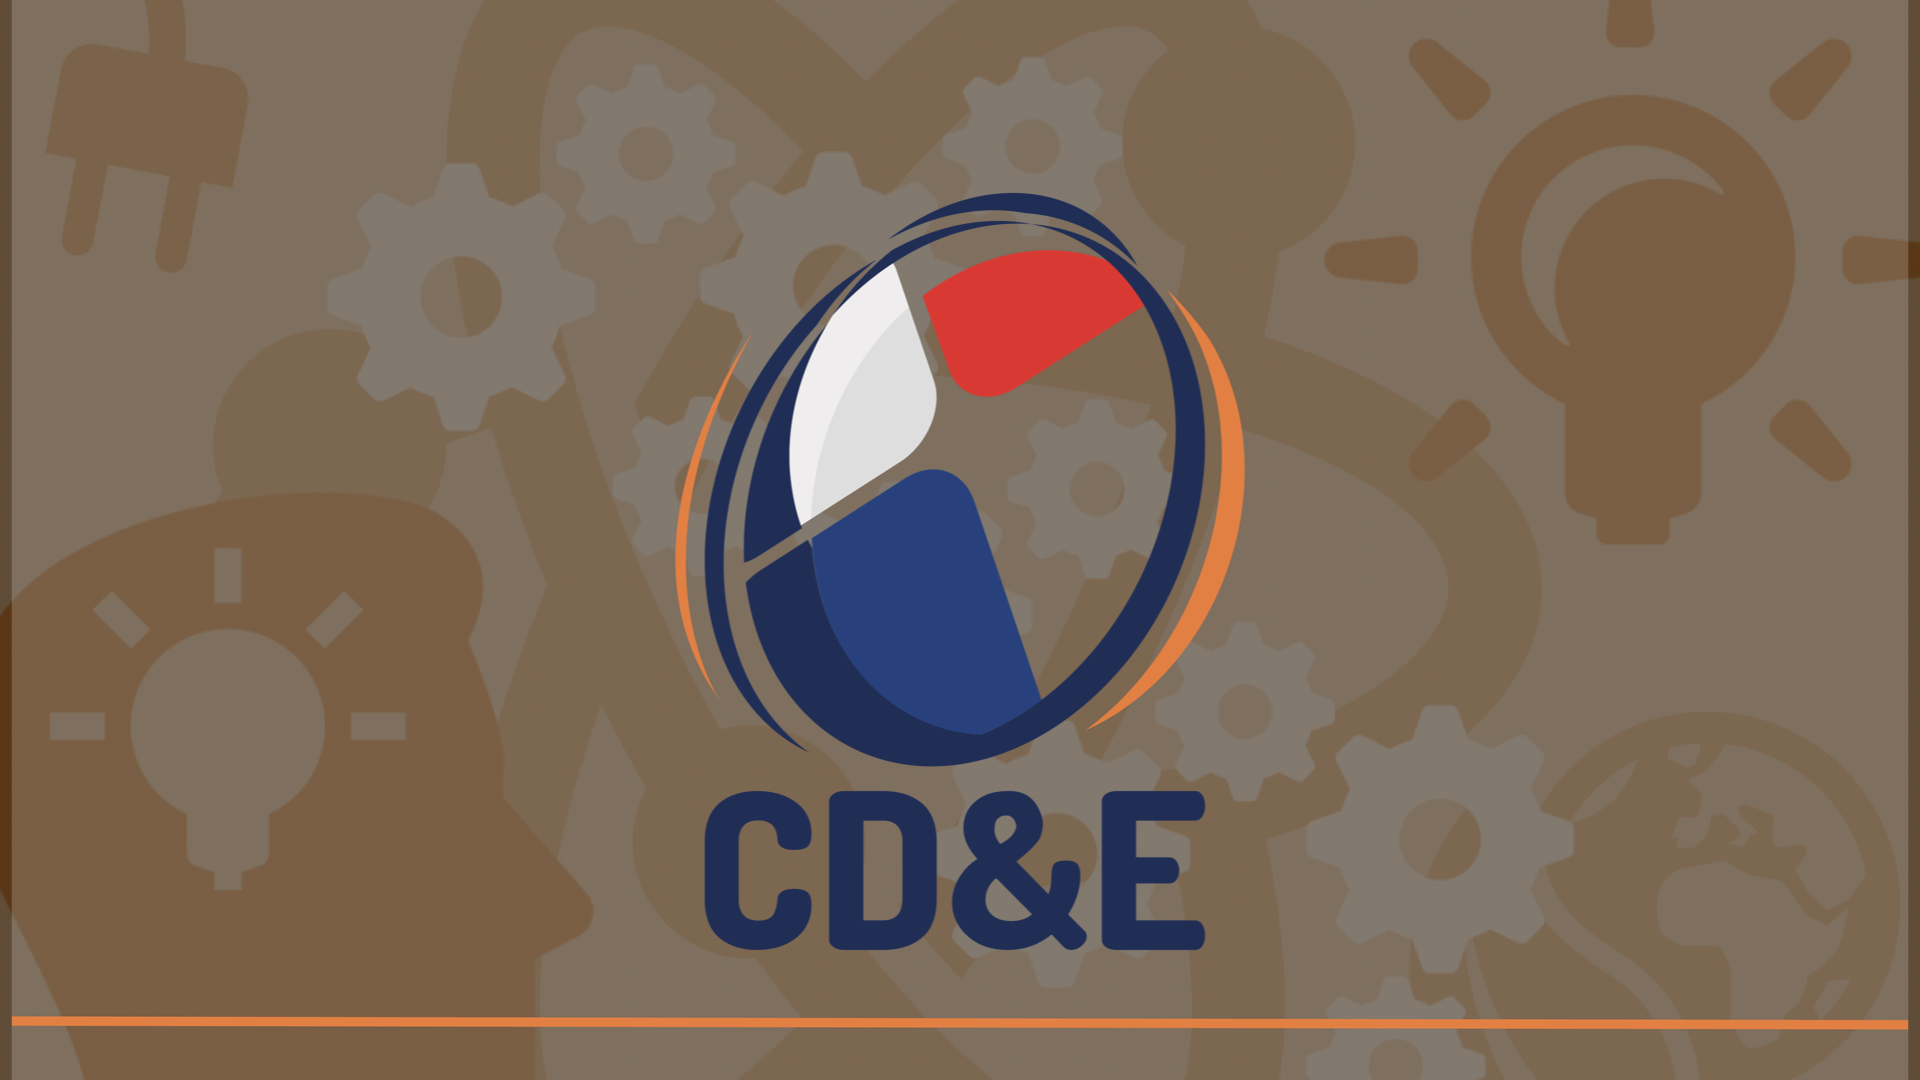
\includegraphics[width=0.7\linewidth]{data/keynote-slides/20200430-CDE-Designprocess/20200430-CDE-Designprocess.001} 

}

\caption{ }\label{fig:unnamed-chunk-2}
\end{figure}

\hypertarget{benaming}{%
\section{benaming}\label{benaming}}

De naam van ons team en methode is een aantal keer veranderd. We stonden bekend als CD\&E en worden op dit moment de Afdeling Innovatie (i.o.) genoemd. Onze methodieken worden weleens benoemd als: CD\&E, kort-cyclisch moderniseren of -innoveren, trajectbegeleiding en programmatische aanpak. Ik zie vooral een \emph{craft} ontstaan waarin deze methodes en onze technieken en tools worden gehanteerd door \emph{craftsman}. Ik noem deze `craft' Military Design \& Innovation. Dit boek beschrijft wat ik onder deze \emph{craft} versta.

\hypertarget{aanleiding}{%
\section{aanleiding}\label{aanleiding}}

De reden om als Landmacht te innoveren met externe partners ligt in de realiteit dat een leger altijd beter moet zijn dan de tegenstander maar legers niet langer de innovatie aanjagen. De markt en economische marktwerking heeft dit overgenomen. En daar waar de Landmacht het idee had de ontwikkelingen voldoende te kunnen volgen, kreeg de Commandant Landstrijdkrachten de spiegel voorgehouden door de voorzitter/directeur van werkgeversorganisatie FME-CWM tijdens de Future Force Conference in 2015. De Landmacht pakte deze reflectie serieus aan en zoekt met externe organisaties naar samenwerking om in het tempo van de markt te innoveren in het landoptreden. De Landmacht gebruikte hierbij ondermeer de methode Concept Development \& Experimentation (CD\&E) als startpunt voor deze zoektocht.

CD\&E starte in 2015 als zogenaamde kwartiermakersgroep en maakte naam als afdeling, methode en resources voor kort cyclische moderniseren in het landoptreden. Sinds oktober 2017 mag ik bijdragen aan de missie van CD\&E. Startend als algemeen stafofficier junior ontwikkelde we met een klein team een methode, proces, tools en concept waarmee we kenniscentra en parate eenheden in staat konden stellen hun ideeën, en problemen om te zetten in vraagstukken die samen met interne en externe partijen middels experimenten worden beantwoord en ---als ultieme doel--- formeel opgenomen in de organisatie (implementatie). Deze aanpak is geen nieuw format of procedure maar een continue leerproces waarin samen wordt gewerkt aan nieuwe denkmodellen, activiteiten-pallet en craftmanship.

Veel van de CD\&E-aanpak is door de groei, successen (en mislukkingen) en de omgeving verandert, verbeterd of doorontwikkeld. Ook onstaan er nieuwe methode, processen, tools en concepten die de mogelijkheden voor innovatie in het landoptreden vergroten. Al deze nieuwe inzichten en handelingsperspectieven worden omgezet in kennis en vaardigheden die worden geborgt en gedeelt. Deze inspanningen dragen daarmee bij aan onze missie.

\hypertarget{missie}{%
\section{missie}\label{missie}}

\begin{quote}
We ontsluiten het innovatieve vermogen van het bedrijfsleven en kennisinstituten voor het moderniseringsproces van de Land- en/of Krijgsmacht zodat onze eenheden tijdens inzet relevant en waar nodig dominant blijven.
\end{quote}

In het vakgebied Military Design \& Innovation borgen en delen we de kennis en vaardigheden die ruimte bieden aan nieuwe manieren om innovatie bij de Landmacht integraal, experimenteel en in steeds hoger tempo met externe partijen uit te voeren.

\hypertarget{beleid}{%
\section{beleid}\label{beleid}}

\begin{figure}

{\centering 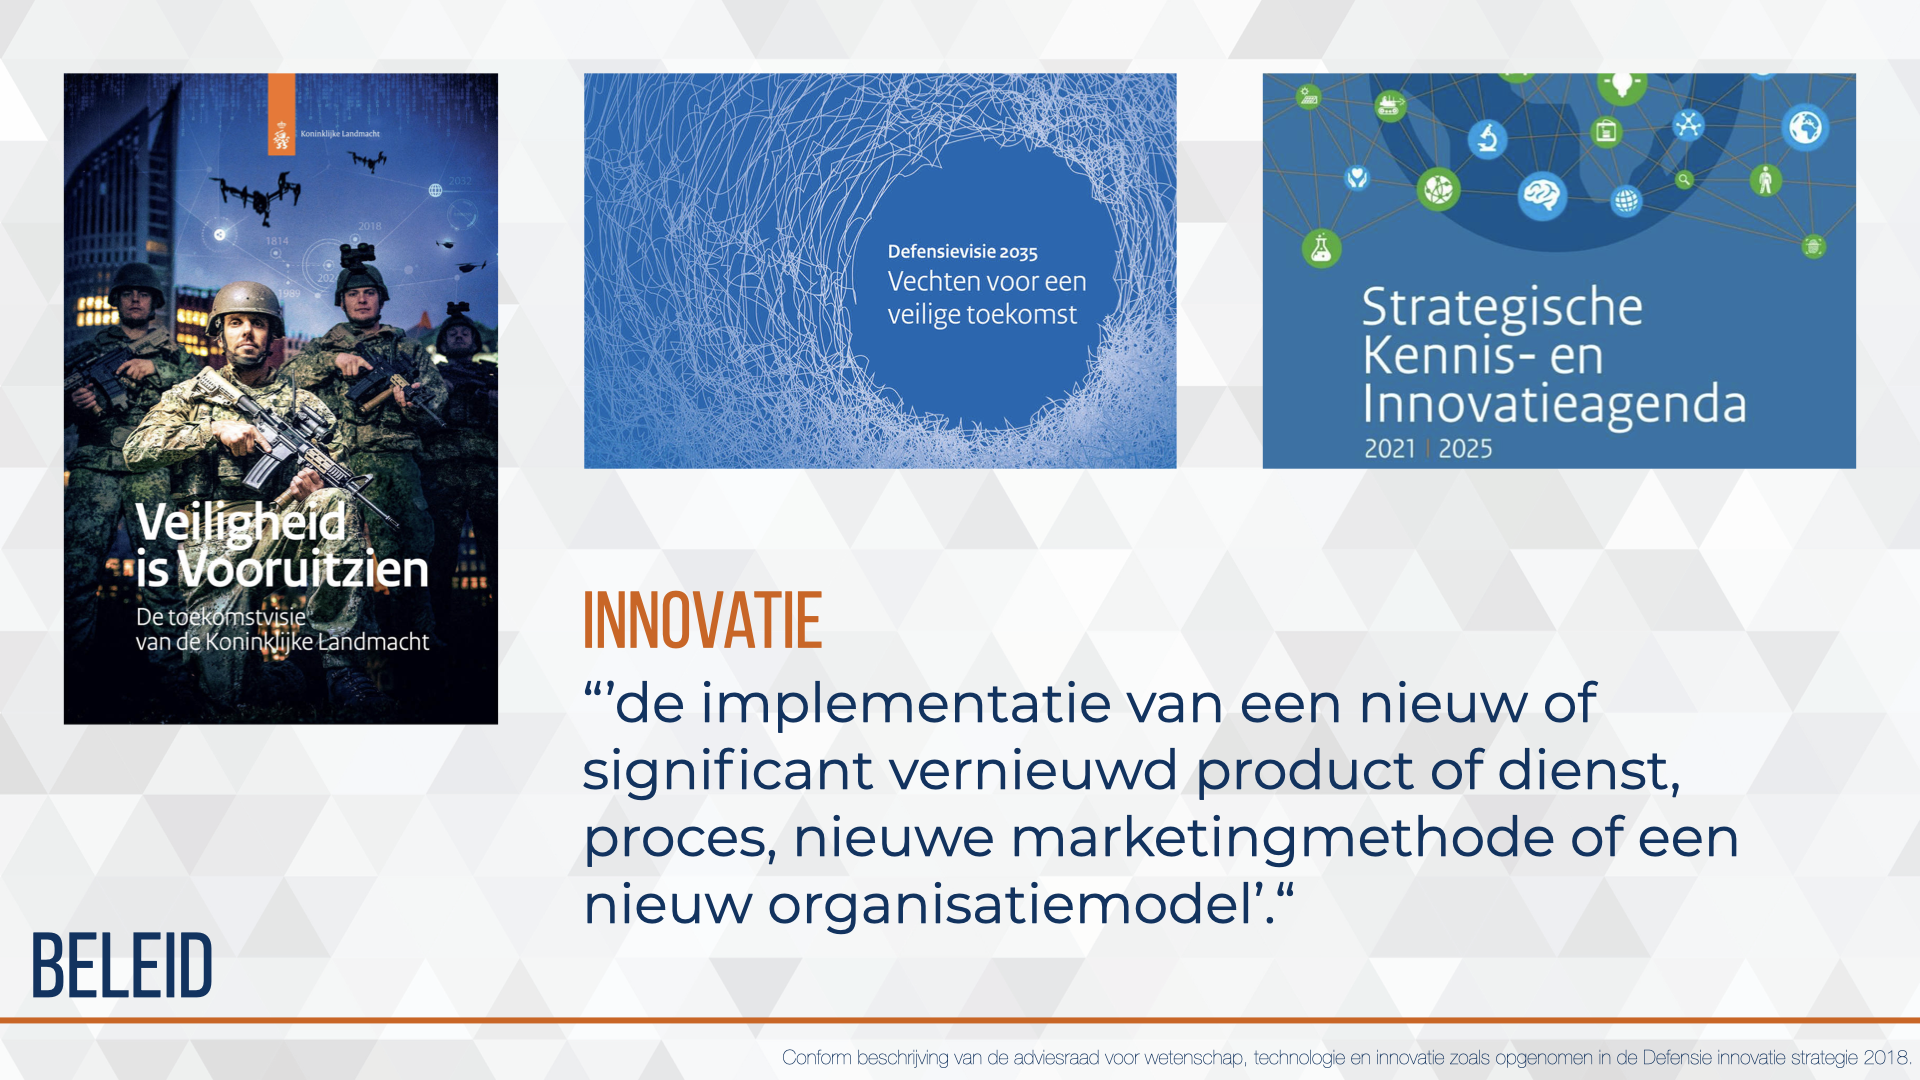
\includegraphics[width=0.7\linewidth]{data/keynote-slides/20200430-CDE-Designprocess/20200430-CDE-Designprocess.005} 

}

\caption{ }\label{fig:unnamed-chunk-3}
\end{figure}

Er zijn een aantal beleidsdocumenten die het moderniseren en innoveren van de Land- en Krijgsmacht sturen. Drie documenten komen met enige regelmaat terug. De Defensievisie 2035, Vechten voor een veilige toekomst beschrijft de inrichtingsprincipes voor de eerstkomende jaren. De Strategische kennis- en innovatieagenda geeft meer thematisch aan in welke onderwerpen Defensie de focus legt. De Visie Commando Landstrijdkrachten, Veigligheid is vooruitzien, beschrijft het toekomstbeeld van de Kominklijke Landmacht. Deze is intern verder vertaald in het Operationeel kader landoptreden (OKL).

Als definitie voor innovatie volgen we de Adviesraad voor Wetenschap, Technologie en Innovatie.

\begin{quote}
Innovatie: ``de implementatie van een nieuw of significant vernieuwd product of dienst, proces, nieuwe marketingmethode of een nieuw organisatiemodel.`` (\protect\hyperlink{ref-awti-2014}{Adviesraad voor het Wetenschaps- en Technologiebeleid, 2014})
\end{quote}

\hypertarget{uitgangspunten}{%
\section{uitgangspunten}\label{uitgangspunten}}

Bij het ontwikkelen van een modellen en processen moet Defensie met een aantal zaken rekening houden. Bij wet kent Defensie --en dus ook de Landmacht-- een aantal verplichtingen zoals de wijze waarop partners en leveranciers worden geselecteerd of de manier waarop geld wordt uitgegeven.

Daarnaast kent de organisatie een snelle doorstroom van functionarissen en dwingende processen en regels.
Functionarissen doen wat zij kennen, weten en wat de afdeling of eenheid gewoon is te doen vanuit de intentie kwaliteit te willen leveren als vakmensen. Door de snelle doorstroom is het lastig de mogelijkheden van de wet- en regelgeving ten volle te benutten.
Procedures maken de gang van zaken controleerbaar, repeteerbaar en voorspelbaar maar vooral borgt het de sociale waarden van de Landmacht als overheidsorganisatie.

Dit resulteert in drie uitgangspunten die kaderstellend zijn bij het doorontwikkelen van modellen, processen en instrumenten voor Military Design \& Innovation.

\textbf{Landmacht is een aanbestedende dienst}
dus moeten inkoop en verwerving voldoen aan Europese wetgeving.

\textbf{Landmacht is een rijksoverheidsorganisatie}
met een Ministeriële verantwoording aan parlement over verantwoorde uitgave van belastinggeld en handelen naar de Nederlandse overtuigingen en belangen.

\textbf{Landmacht is een bureaucratische organisatie}
waarin processen en regelgeving borgen dat de organisatie non-discriminatief handelt conform Weber's model.

\hypertarget{moderniseringsmodellen}{%
\section{moderniseringsmodellen}\label{moderniseringsmodellen}}

Voor de lang-cyclische modernisering kent de Landmacht het CLAS moderniseringsmodel waar vanuit een future scan (landoptreden van de toekomst LvT) wordt toegewerkt naar een force design (Landmacht van overmorgen LvOM), force building (Landmacht van morgen LvM) en force employment (Landmacht van vandaag LvV).

\begin{figure}

{\centering 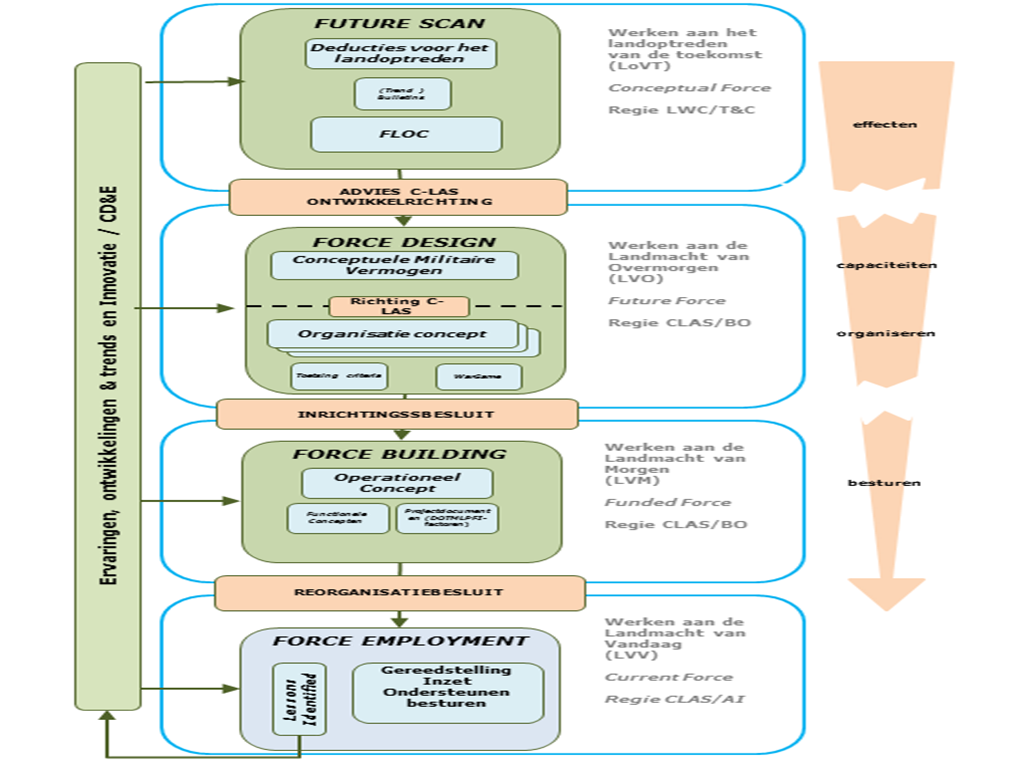
\includegraphics[width=14.29in]{data/images/BO-2016-CLAS-moderniseringsmodel} 

}

\caption{CLAS moderniseringsproces lang-cyclisch }\label{fig:unnamed-chunk-4}
\end{figure}

Defensie breed is de lang-cyclische modernisering en innovatie ingericht als een `huis'. Dit kennis- en innovatie model is al jaren in gebruik en voorziet in vele instrumenten en processen om innovatie op lange termijn toe te passen. Echter het gebruiken van nieuwe snel opkomende innovaties kunnen hiermee niet adequaat worden getest en geïmplementeerd.

\begin{figure}

{\centering 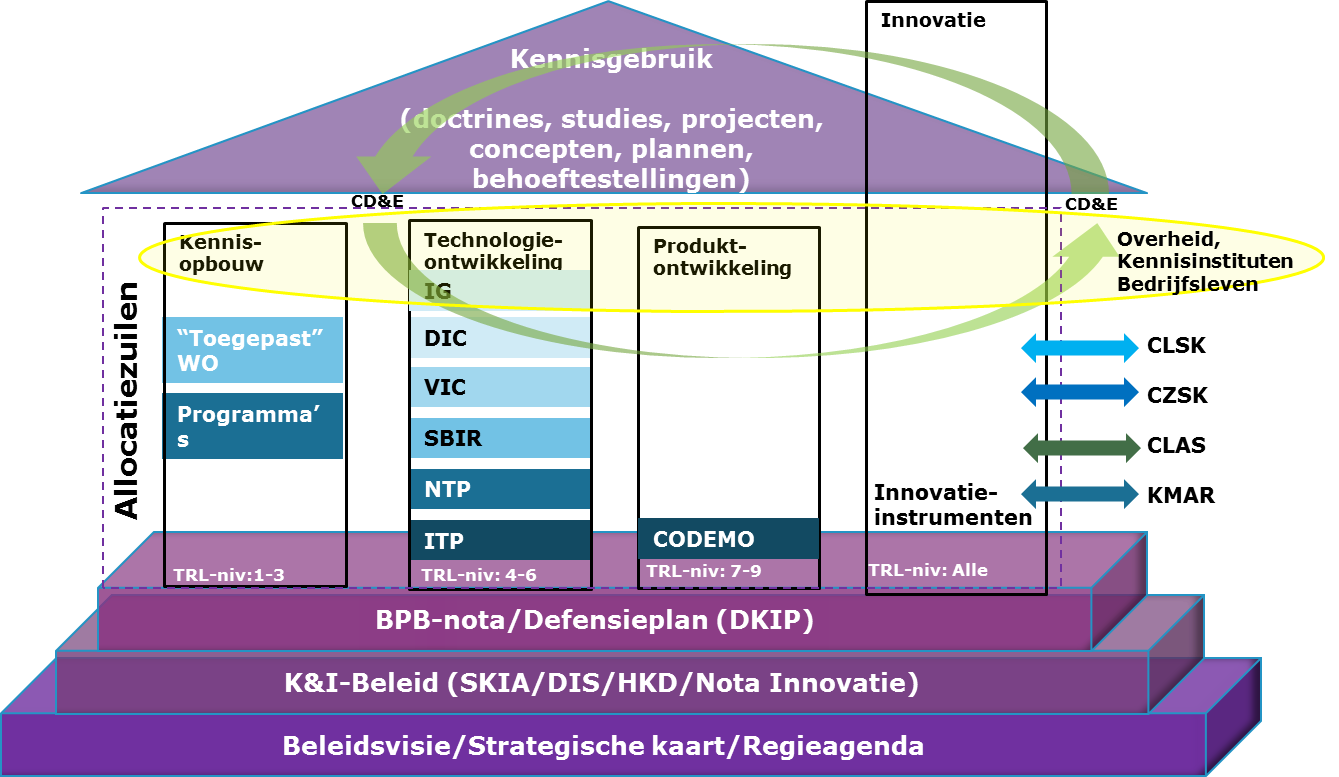
\includegraphics[width=0.7\linewidth]{data/images/BO-2016-Defensie-KI-huis} 

}

\caption{Visuele weergave van het kennis \& innovatiehuis Defensie}\label{fig:ki-test}
\end{figure}

Met CD\&E werkt de Landmacht sinds 2015 aan het versnellen, verbinden en vermarkten van opkomende technologieën en ambities door het organiseren en structureren van innovatie in het tempo van de markt.

\hypertarget{cde-binnen-clas-modernisering}{%
\subsection*{CD\&E binnen CLAS-modernisering}\label{cde-binnen-clas-modernisering}}
\addcontentsline{toc}{subsection}{CD\&E binnen CLAS-modernisering}

\begin{figure}

{\centering 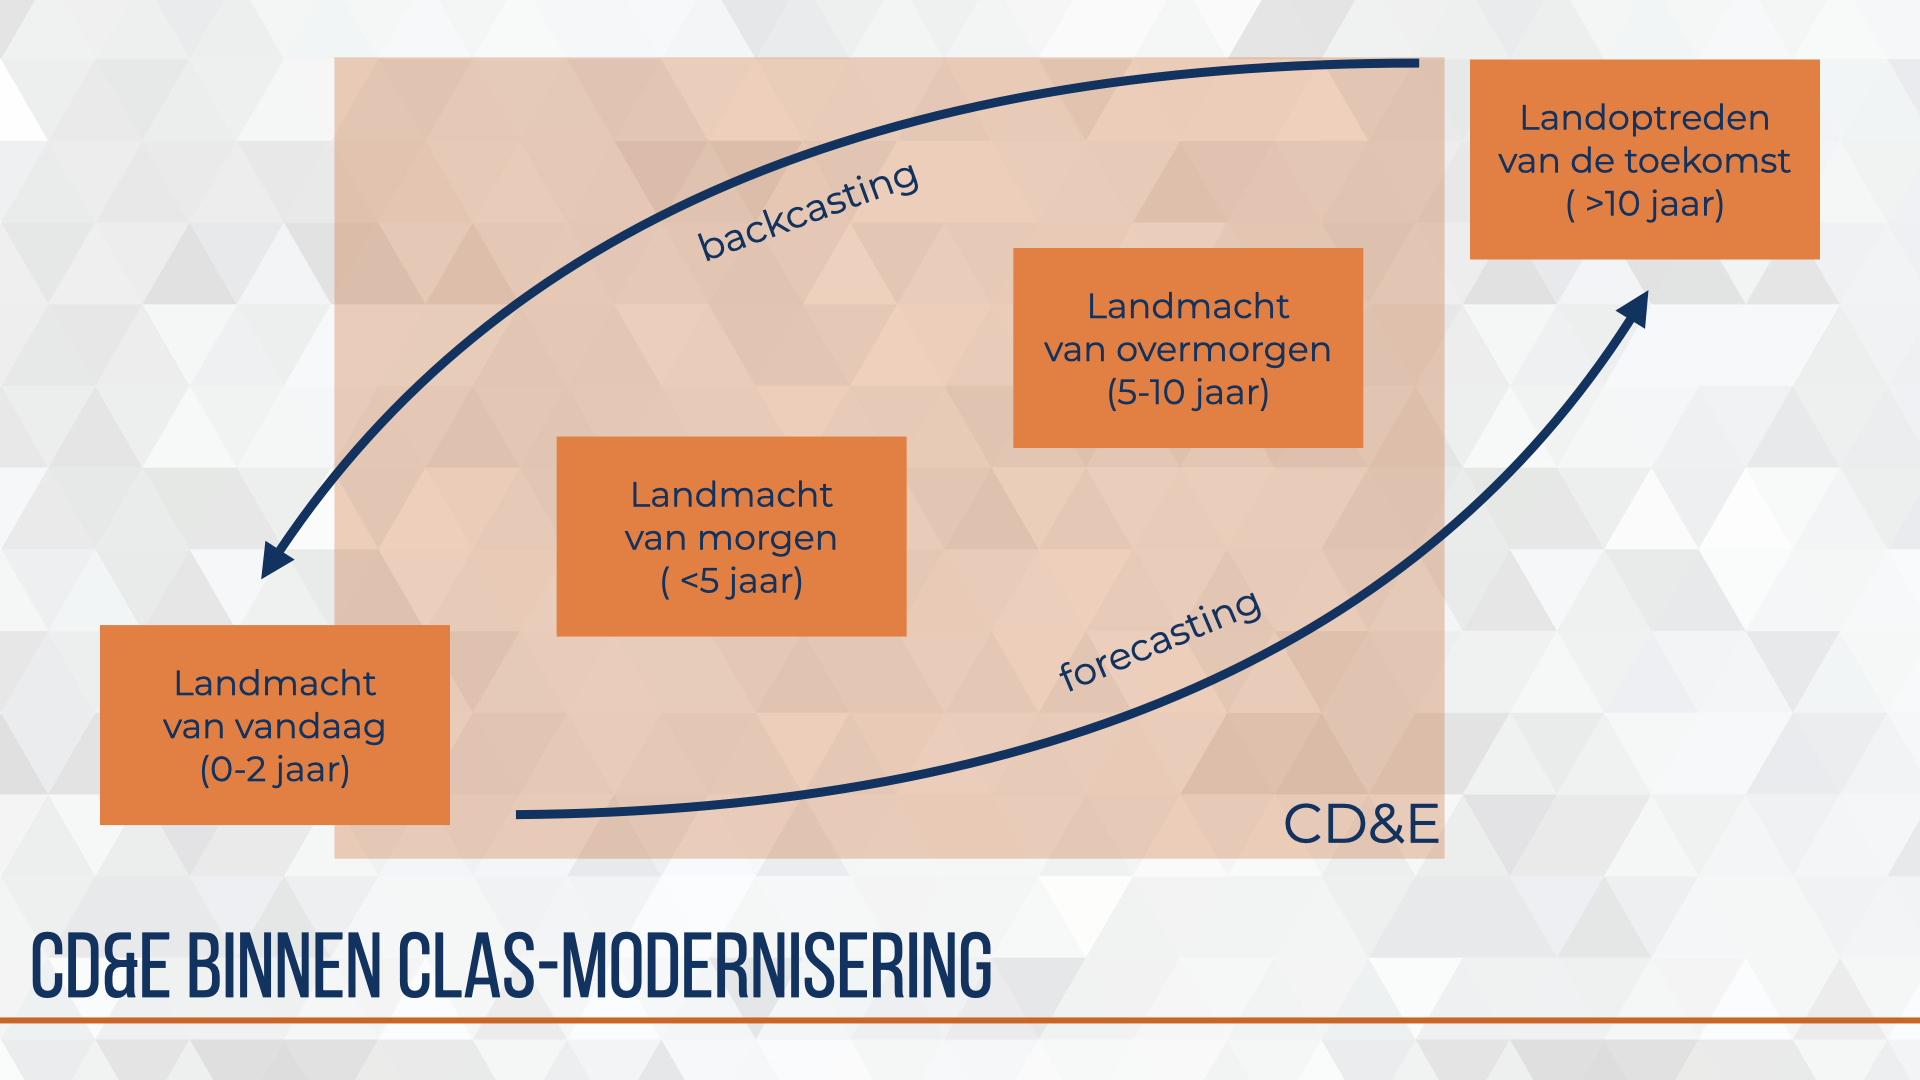
\includegraphics[width=0.7\linewidth]{data/keynote-slides/20200430-CDE-Designprocess/20200430-CDE-Designprocess.008} 

}

\caption{Eenvoudig CLAS moderniseringsproces met positionering van de CD\&E-methodiek}\label{fig:simpel-proces}
\end{figure}

Figuur @ref((fig:simpel-proces)) en vereenvoudigde visualisatie van het `klassieke' moderniseringsproces van de Landmacht. Dit proces kan worden onderverdeeld in vier aandachtsgebieden, de landmacht van vandaag (LvV), morgen (LvM), overmorgen (LvOM) en het landoptreden van de toekomst (LvT). Verschillende organisatie-onderdelen dragen bij aan deze aandachtsgebieden. Grofweg kan de verantwoordelijkheid (responsibility) worden toebedeeld aan respectievelijk de parate eenheid, afdeling strategie \& plannen, kenniscentrum en afdeling trends \& concepts. CD\&E draagt hoofdzakelijk bij aan de landmacht van morgen en overmorgen.

In dit moderniseringsproces onderscheiden we twee bewegingen, backcasting en forcasting. Backcasting vindt plaats doordat onderzoek, studies en verkenningen richting geven aan modernisering voor LvM en LvV. Forecasting vindt plaats doordat evaluaties, lessons learned en experimenten richting geven aan beleid, budgettering en kennisplanning. Beide bewegingen komen terug in Military Design \& Innovation.

\hypertarget{cde-algemeen}{%
\chapter{Organisatie}\label{cde-algemeen}}

De Krijgsmacht moet goed getraind zijn en gedegen uitgerust worden. Het Ministerie van Defensie draagt zorg voor de ontwikkeling, gereedheid en waar nodig inzet van de Krijgsmacht.

Op basis van toekomst verkenningen, veiligheidsscenario's, strategische- en operationele concepten en mogelijke toekomstige operationele omgevingen (MTO's) wordt richting gegeven aan het Krijgsmacht ontwikkelproces. Met beleidsplannen worden de benodigde capabilities gededuceerd, budgetten gealoceerd en middelen verworven. Als deze middelen worden samengebracht met mensen in een eenheid met specifieke taken is dit een militaire capaciteit.

De innovatievraagstukken gaan --ondermeer-- over de ontwikkelingen die niet voorzienbaar of planbaar zijn in de BPB-cycli \footnote{beleid, begroot en plan cylci} van het Kerndepartement. De nieuwe manieren die de Afdeling Innovatie nastreeft zijn daarom aanvullend op de bestaande manieren voor ontwikkeling van de Krijgsmacht. Waar mogelijk gebruiken we bestaande programma's, projecten, processen en instructies. Hierdoor maken we optimaal gebruik van bestaande capaciteiten en middelen om de Krijgsmacht altijd technologisch hoogwaardig inzetbaar te houden.

\hypertarget{positionering-in-defensie-organisatie}{%
\section{positionering in defensie organisatie}\label{positionering-in-defensie-organisatie}}

\begin{figure}

{\centering 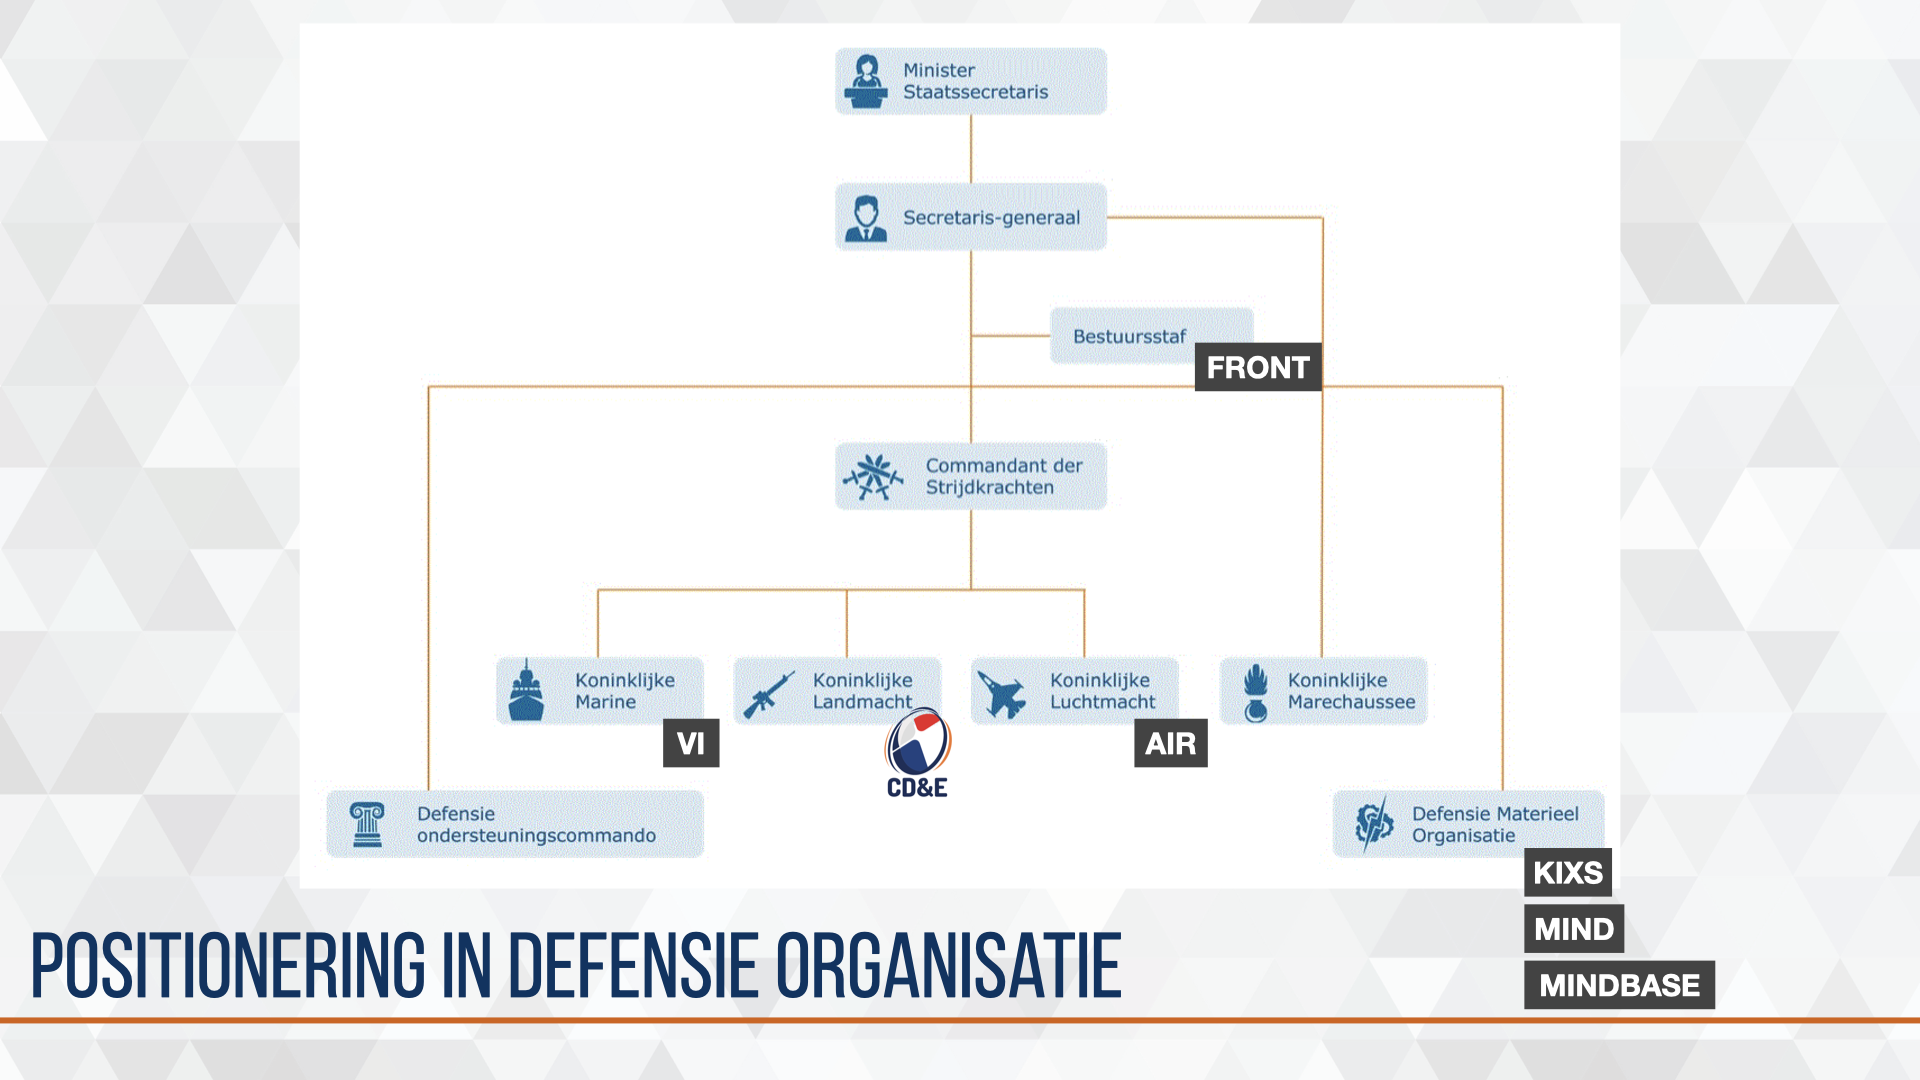
\includegraphics[width=0.7\linewidth]{data/keynote-slides/20200430-CDE-Designprocess/20200430-CDE-Designprocess.009-1} 

}

\caption{Positionering innovatiecentra binnen Defensie }\label{fig:unnamed-chunk-6}
\end{figure}

CD\&E is het innovatiecentrum van de Landmacht. Ook de andere defensieonderdelen kennen innovatiecentra, ieder opgebouwd in de kenmerken en cultuur van het defensieonderdeel.

\begin{quote}
De content van dit hoofdstuk wordt herschreven naar een globale introductie van het Krijgsmacht Ontwikkelproces van Defensie en het Commando Landstrijdkrachten. Neem contact met mij op voor de actuele informatie.
\end{quote}

\hypertarget{how-to-think}{%
\chapter{How to think}\label{how-to-think}}

De Landmacht is een rijksoverheidsorganisatie die -waar nodig- een zwaardmacht moet zijn op plekken waar vrede en veiligheid geen vanzelfsprekendheid is. Vanuit de grondwettelijke taken is afgeleid hoe de Landmacht optreedt, welke materieel en personele middelen daarvoor nodig zijn en hoe dit wordt georganiseerd. Deze lineaire denkmodellen dragen decenia lang bij aan de innovatie in het landoptreden. De bestaande Landmacht organisatie is in een continue verbeter modus vanuit deze volgordelijkheid.

De technologische en sociale innovaties gaan echter zo snel dat ook op andere, snellere manieren wordt gekeken naar modernisering van de bestaande organisatie en vernieuwing voor de toekomstige organisatie. Military Design \& Innovation geeft nieuwe manieren om innovatie bij de Landmacht uit te voeren in het tempo van de markt. Centraal staat daarbij een integrale aanpak met externe partijen.

Nieuwe manieren vragen om anders denken en doen dan we gewend waren. In dit hoofdstuk beschrijven we een aantal relevante denkmodellen en enkele terminologie om die gezamenlijke veranderopgaaf te ondersteunen.

\hypertarget{effectbrenger}{%
\section{effectbrenger}\label{effectbrenger}}

\begin{figure}

{\centering 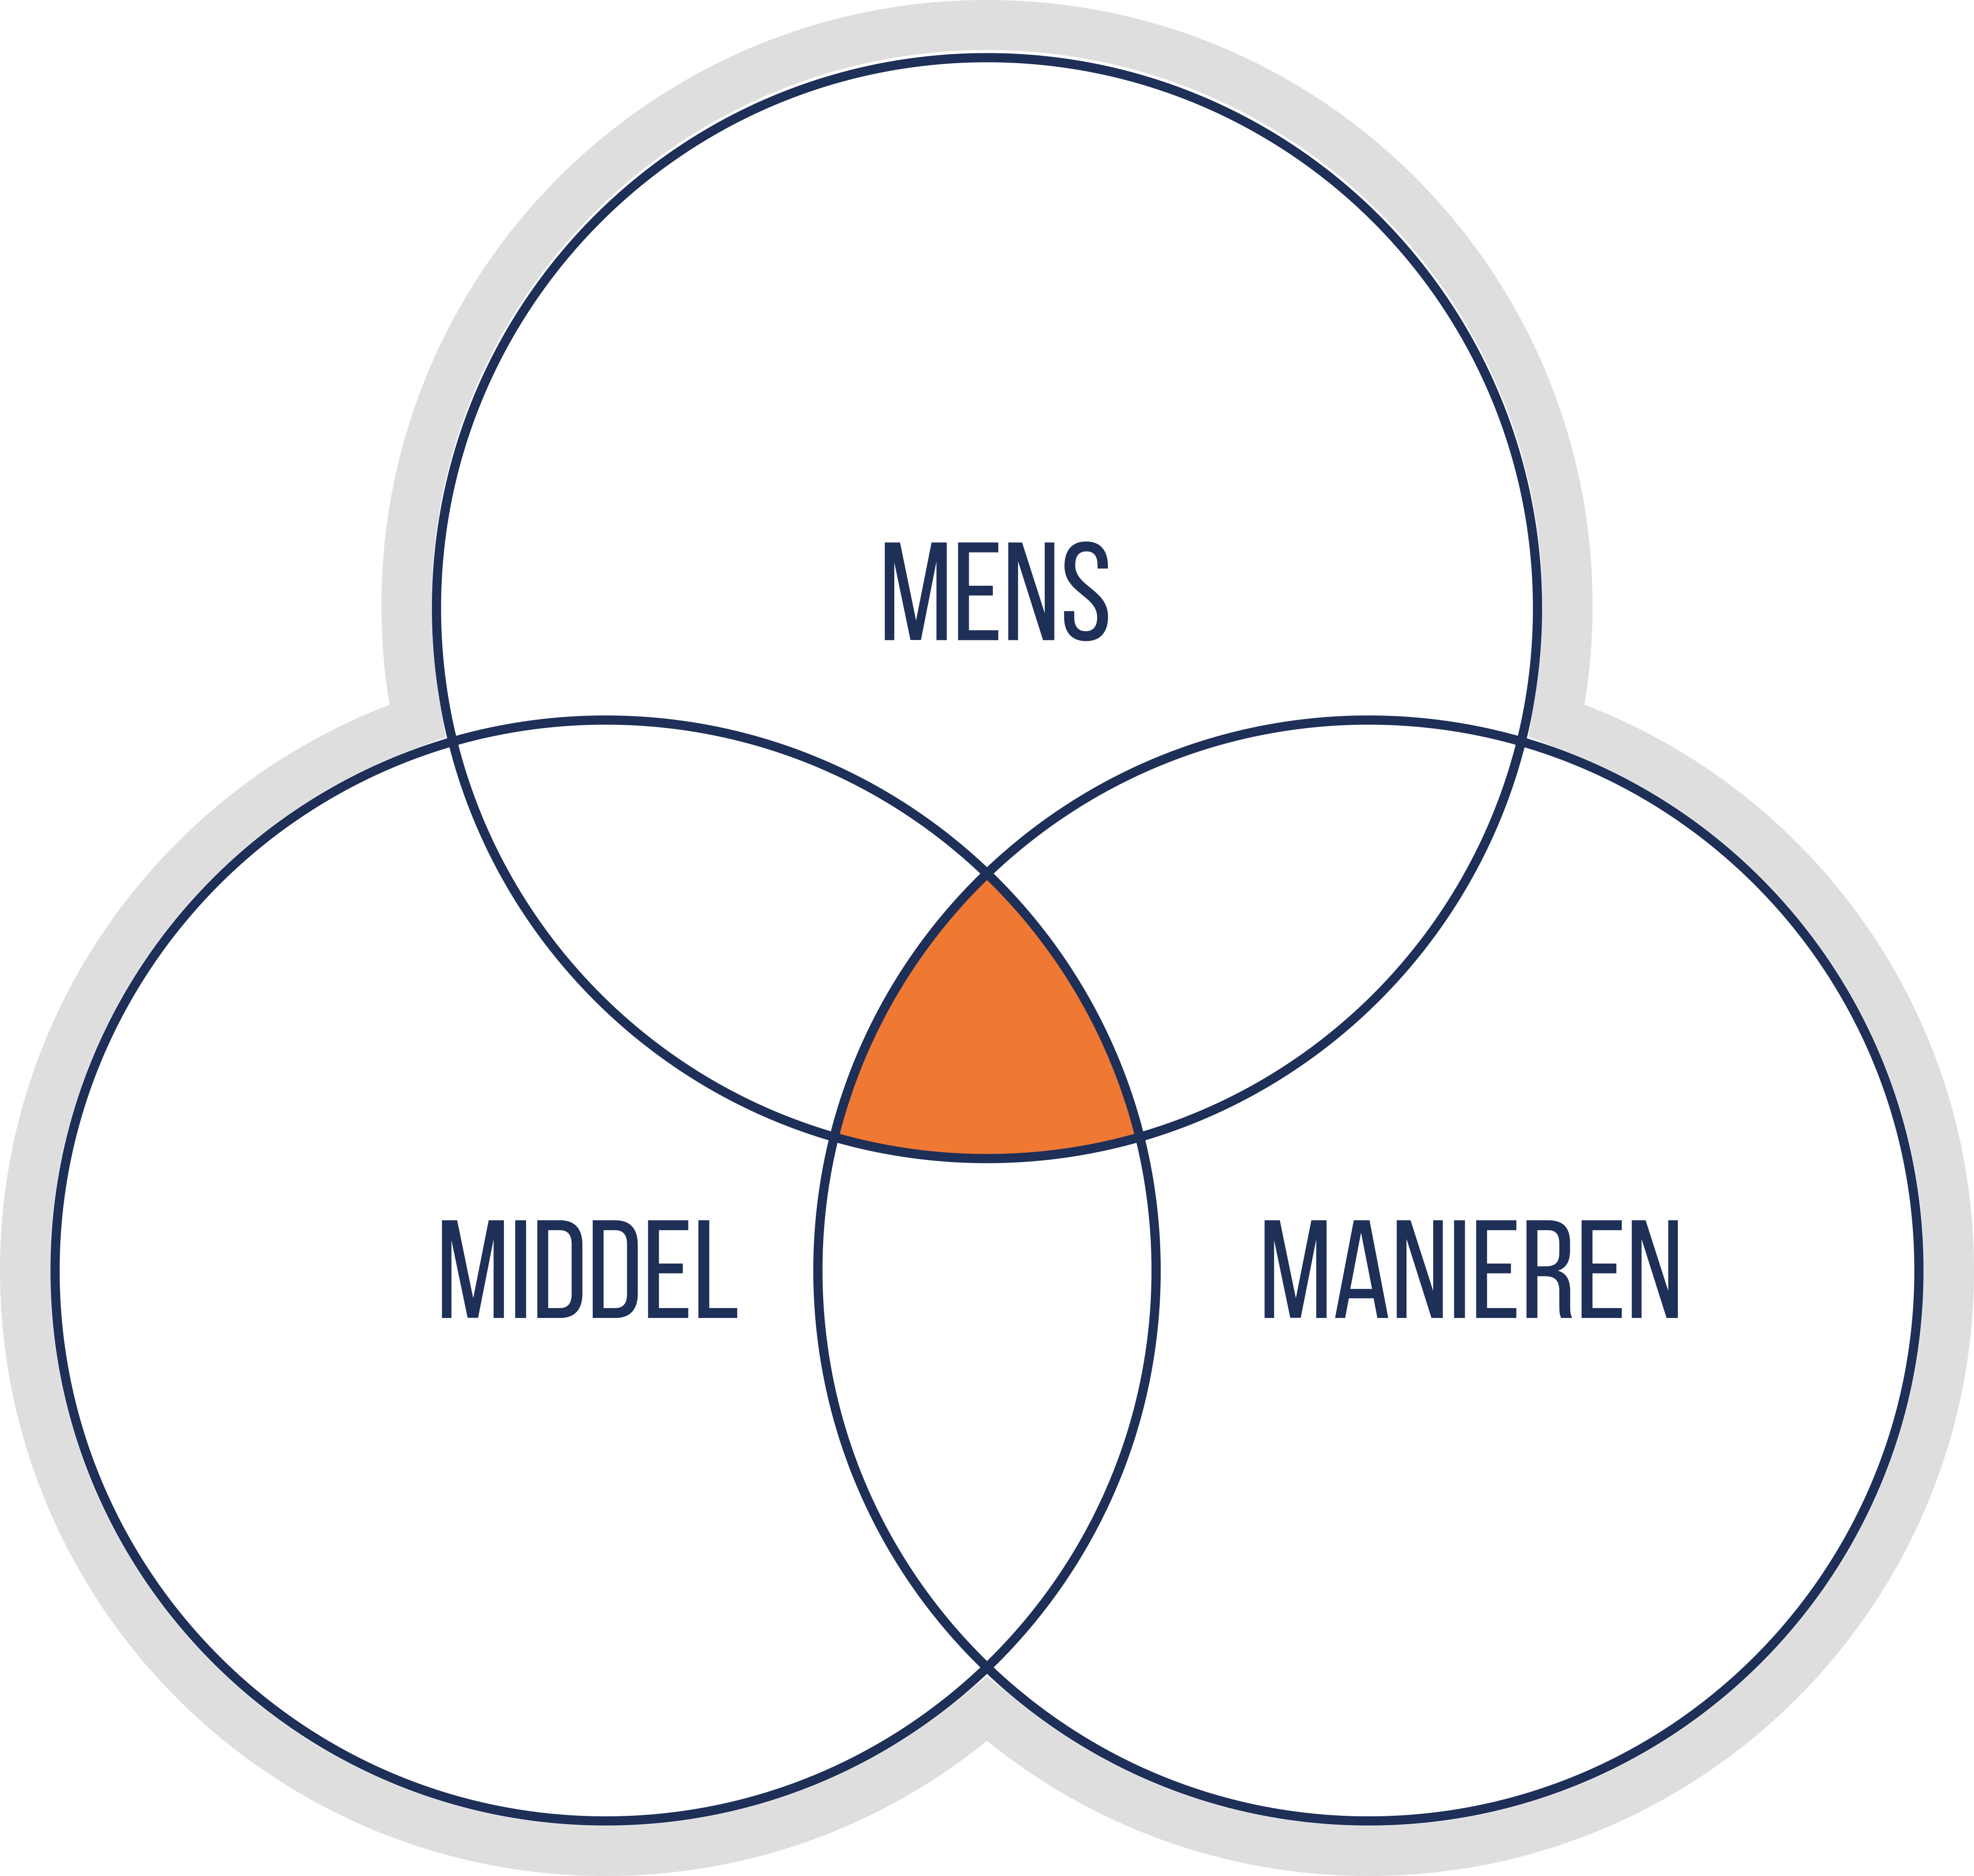
\includegraphics[width=0.35\linewidth]{data/images/20210324-MDI-mmm-model} 

}

\caption{De unieke combinatie van mens, manier en middel maakt een effectbrenger.}\label{fig:mmm-model}
\end{figure}

Een military capability, organisatie onderdeel of subsysteem is een unieke combinatie van mens, manieren en middel(en). Deze unieke combinatie noemen we een effectbrenger.

\begin{figure}

{\centering 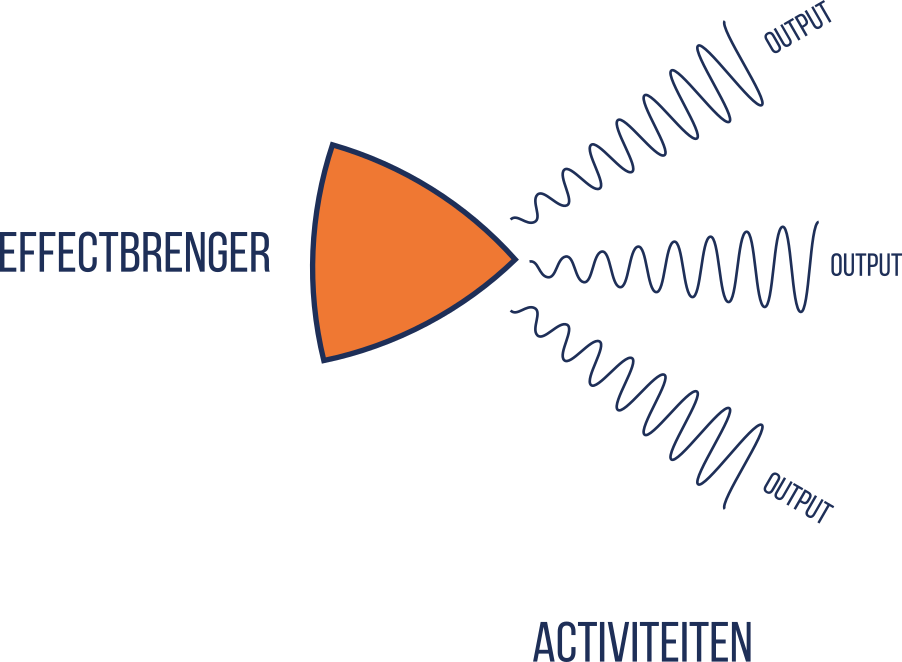
\includegraphics[width=0.45\linewidth]{data/images/20210324-MDI-effectbrenger} 

}

\caption{Een effectbrenger genereert activiteiten met een specifieke output.}\label{fig:effectbrenger}
\end{figure}

Deze effectbrenger voert activiteiten uit met een specifieke, direct te relateren, output. Dit geheel van effectbrenger, activiteiten en output is een zelfstandig en gesloten systeem. De output is afhankelijk van de effectbrenger en activiteiten.

\begin{figure}

{\centering 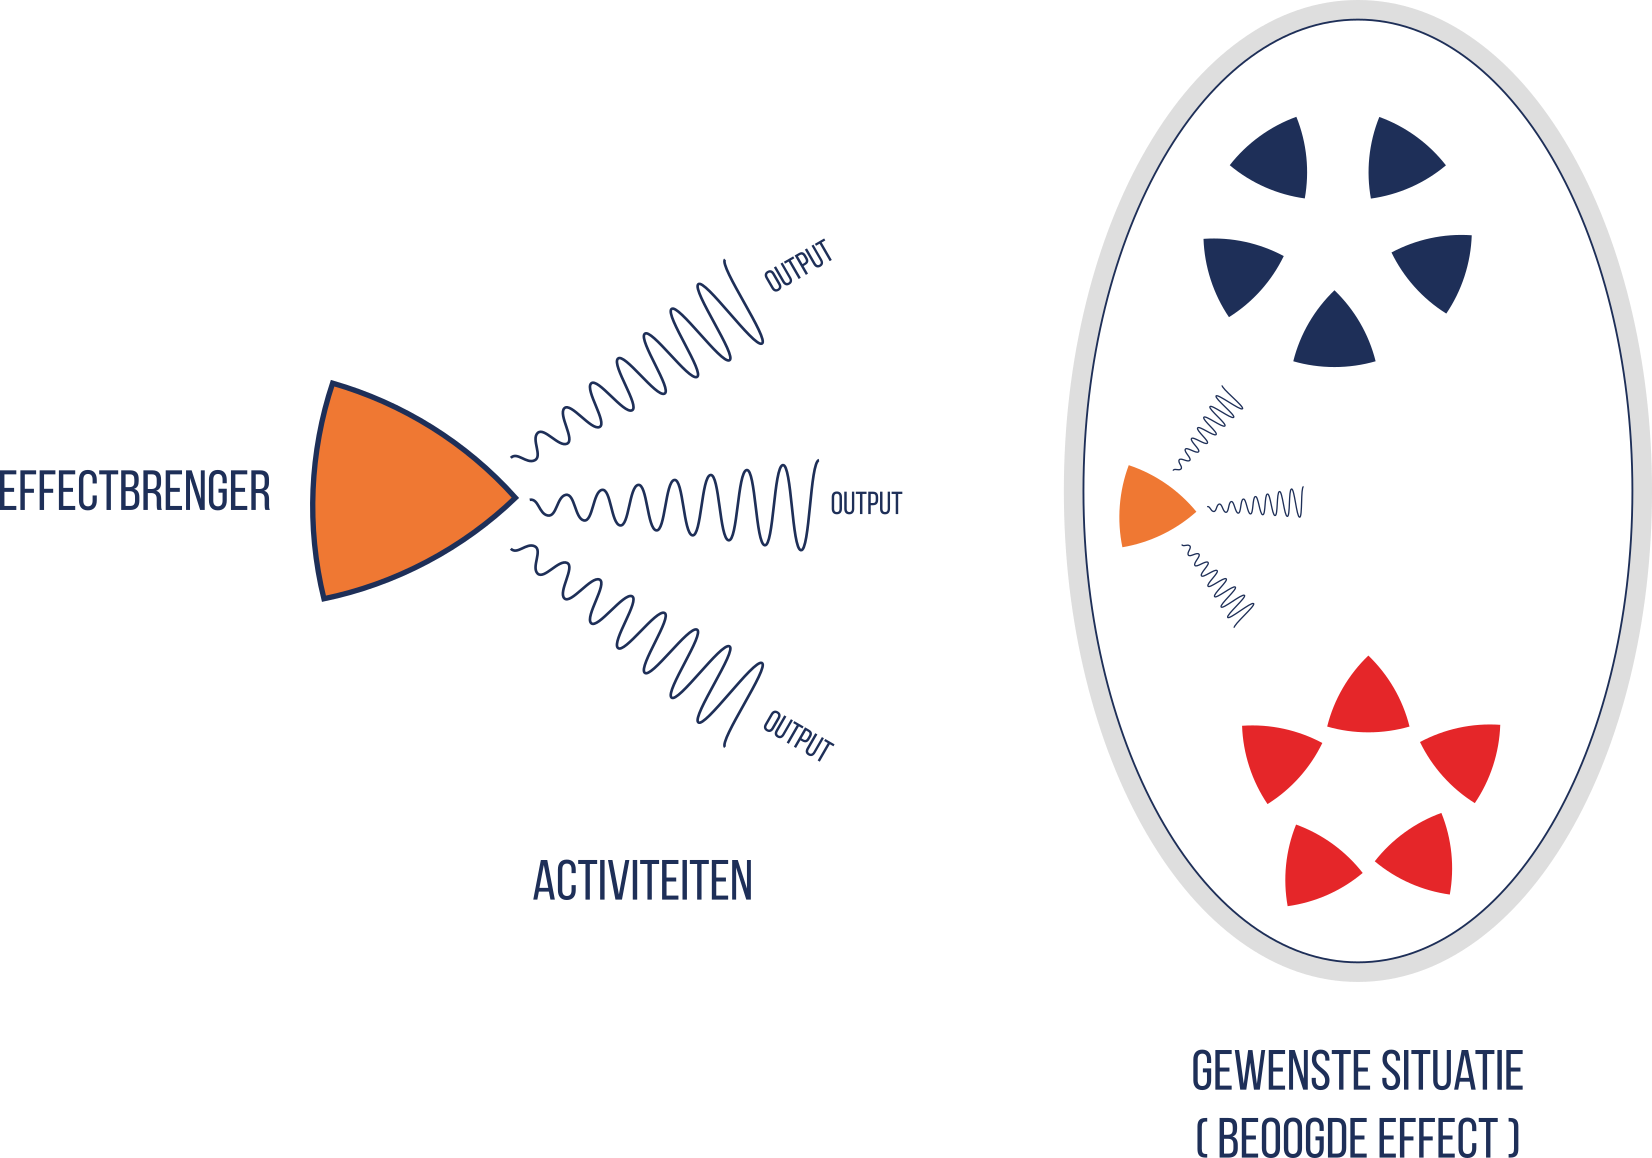
\includegraphics[width=0.45\linewidth]{data/images/20210324-MDI-effectbrenger-ei} 

}

\caption{In een specifieke context creëert een effectbrenger met acitiviteiten en output een effect vanuit de omgeving.}\label{fig:effectbrenger-met-ei}
\end{figure}

\hypertarget{effect}{%
\section{effect}\label{effect}}

De activiteiten en output genereren een reactie in de omgeving, het indirect te relateren, effect. Dit creëert de waarde en impact van de effectbrenger in een specifieke context.

\begin{figure}

{\centering 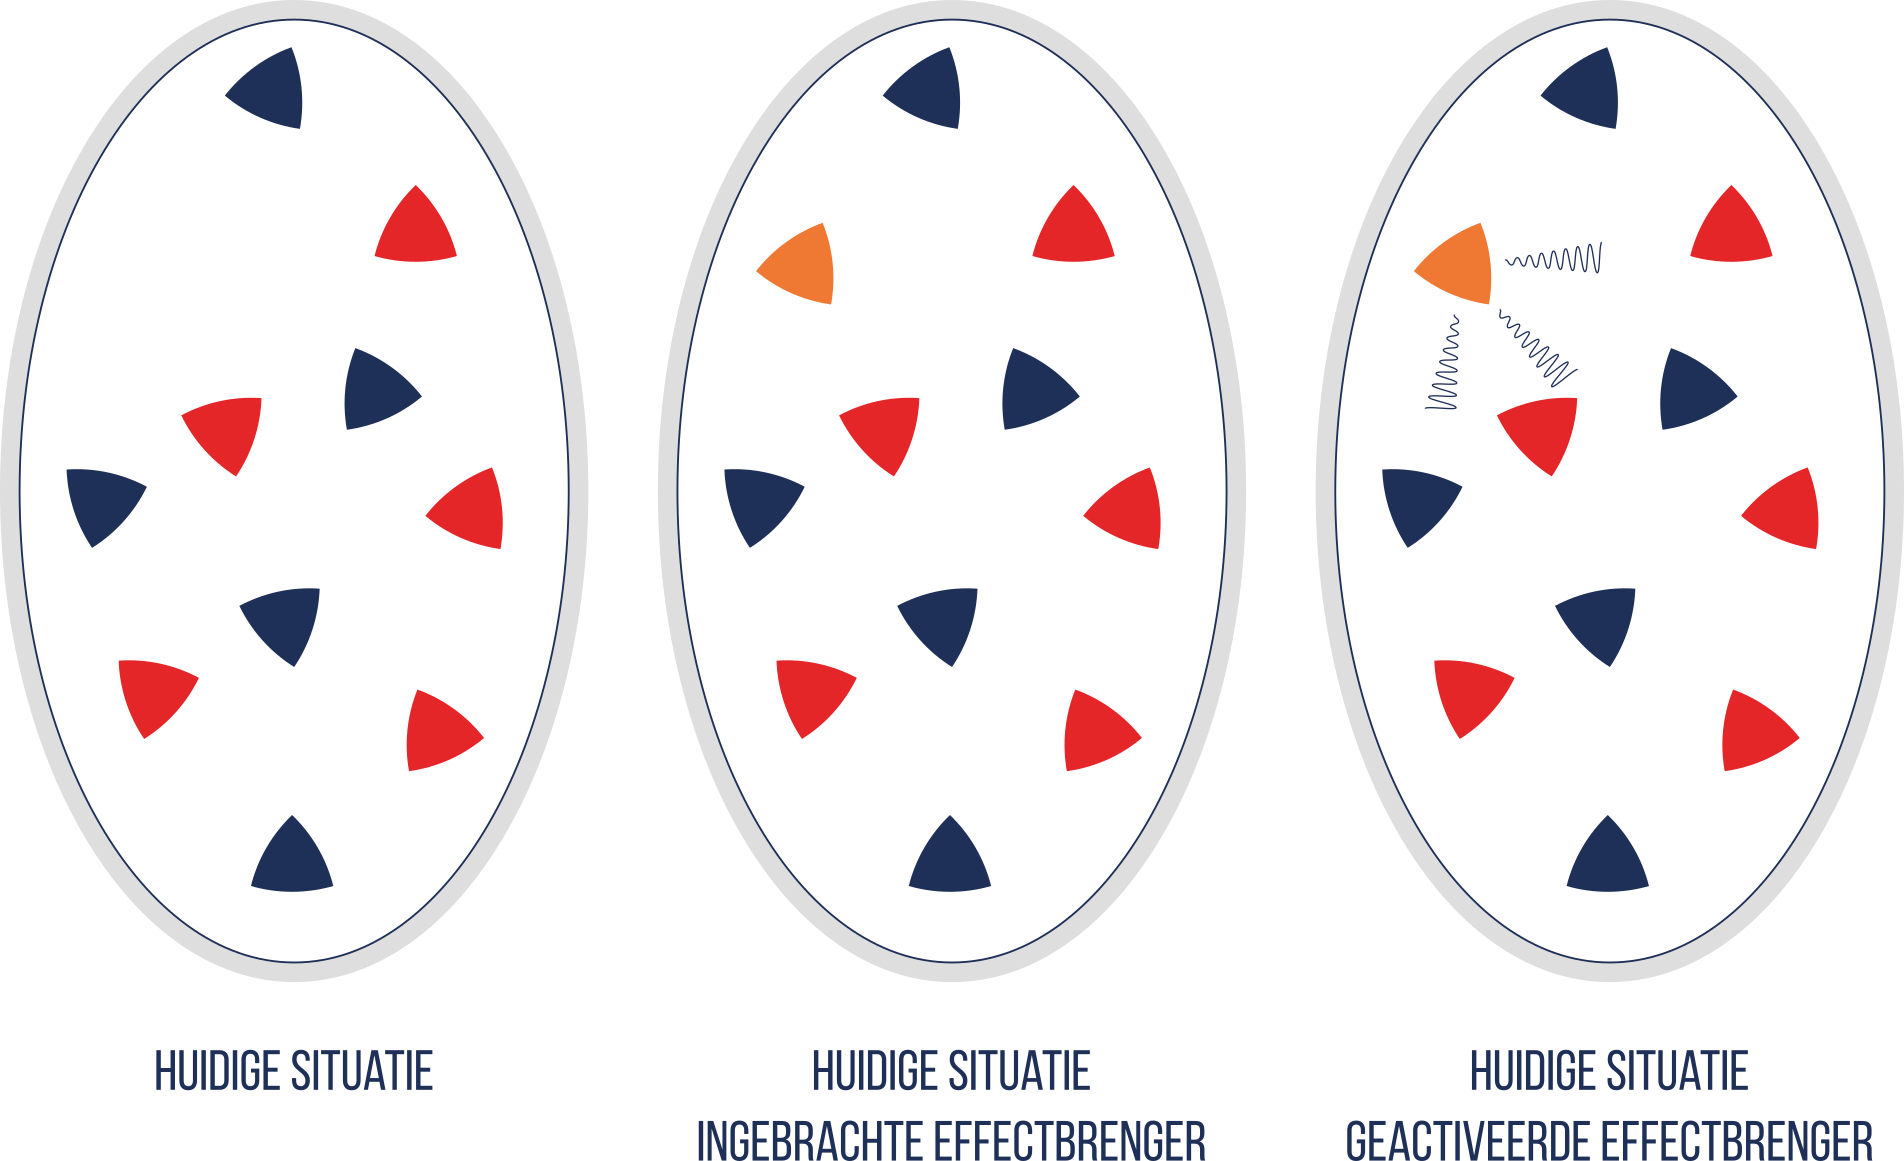
\includegraphics[width=0.85\linewidth]{data/images/20210324-MDI-eieren-huidig} 

}

\caption{Abstracte vormgeving van een specifieke context met een ingebrachte en geactiveerde effectbrenger.}\label{fig:effectbrenger-in-eieren}
\end{figure}

Het feit dat de context veranderd bij het inbrengen of activeren van een effectbrenger is geen causaliteit maar hoogstens een correlatie. Gedegen experimenteren en valideren is daarom van belang.

\hypertarget{context}{%
\section{context}\label{context}}

In de beschrijving van de paragraaf \ref{effect} effecten werd een eerste relatie gelegd met een context. In deze paragraaf \ref{context} worden de soorten context beschreven die regelmatig terugkomen binnen Military Design \& Innovation. Allereerst een kleine `side step' over de betekenis van context.

Oxford Dictionary spreekt over ``The circumstances that form the setting for an event, statement, or idea, and in terms of which it can be fully understood.''(\protect\hyperlink{ref-context}{{``Context,''} n.d.}) en het Van Dale woordenboek definieert context als ``samenhang''. De beschrijving die Military Design \& Innovation --voorlopig-- aanhoudt is:

\begin{quote}
``de plaats- en tijdsgebonden setting van samenhangende relevante actoren en factoren van invloed rondom een specifieke effectbrenger of vraagstuk, bezien vanuit verschillende standpunten, perspectieven en percepties''.
\end{quote}

Hierdoor onstaan twee contexten binnen Military Design \& Innovation. Allereerst de operationele context rondom het design van een vernieuwende operationele capaciteit, en als tweede de organisatie context rondom het innovatietraject wat een idee of ambitie naar implementatie brengt.

\hypertarget{operationele-context}{%
\subsection{operationele context}\label{operationele-context}}

De operationele context is beschrijvend en geeft betekenis aan de opgaaf, eenheid en effectbrenger. Bij het innoveren, moderniseren en transformeren binnen de Koninklijke Landmacht is de setting gedefinieerd als `het landoptreden', zodat de inspanningen gericht blijven op de operationele taak. We onderscheiden hierin de probleem, experimentele en toekomstige context.

\hypertarget{probleem-context}{%
\subsubsection{probleem context}\label{probleem-context}}

\begin{figure}

{\centering 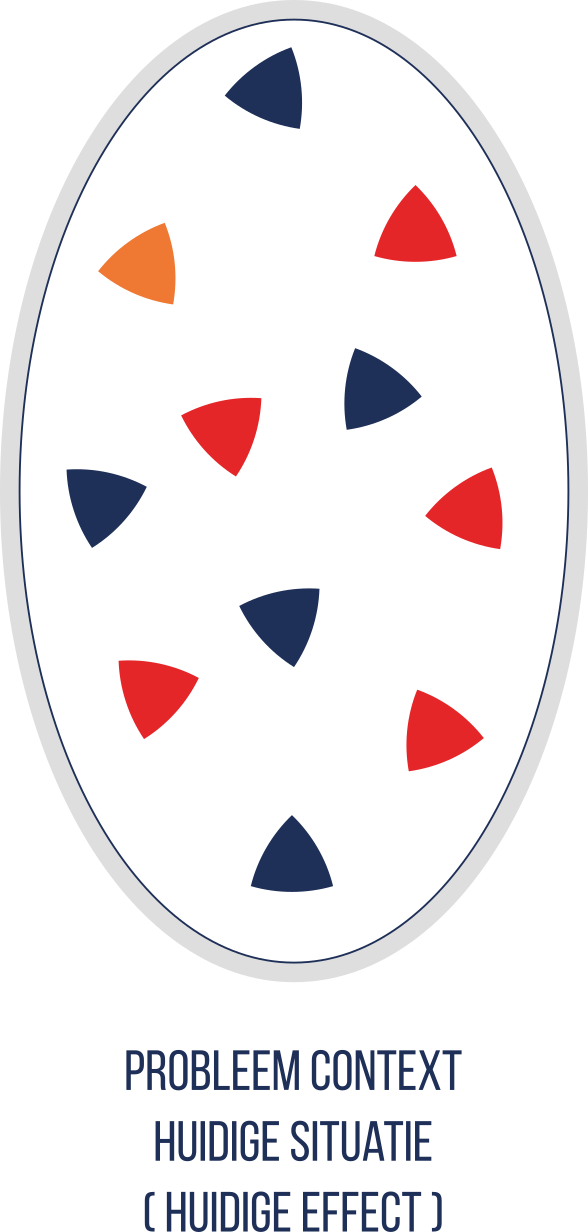
\includegraphics[width=0.2\linewidth]{data/images/20210324-MDI-eieren-beweging-1} 

}

\caption{Abstracte vormgeving van probleem context.}\label{fig:eieren-in-beweging-1}
\end{figure}

In een probleem context beschrijven we de huidige militaire operationele setting van een effectbrenger (militairy capability of eenheid) en beschouwen we een voorgestelde capability gap (operationeel capaciteitsprobleem) of shortfall (operationele tekortkoming). Meestal is sprake van een bestaande effectbrenger die verbeterd wordt, soms wordt een geheel nieuwe effectbrenger ontwikkeld.

Door het opzetten van een probleem context krijgen de betrokken actoren een gemeenschappelijk beeld van de operationele militaire setting waarin het probleem, uitdaging of vraagstuk is ontstaan.

Gezamenlijk plaatsen potentiële partners de opgaaf in de militaire operationele setting. Voor militairen is deze setting `normaal' omdat het hun vakgebied en realiteit is maar voor een niet-militair kan het bijzonder, soms `ver van het bed' en vaak slecht inleefbaar zijn. Dit betekend ook dat militairen blinde vlekken hebben voor de setting en niet-militaire nieuwe inzichten geven. Gezamenlijk werken aan de probleem context verijkt daarmee de vraagarticulatie en aanbodspecificatie.

\hypertarget{toekomstige-context}{%
\subsubsection{toekomstige context}\label{toekomstige-context}}

\begin{figure}

{\centering 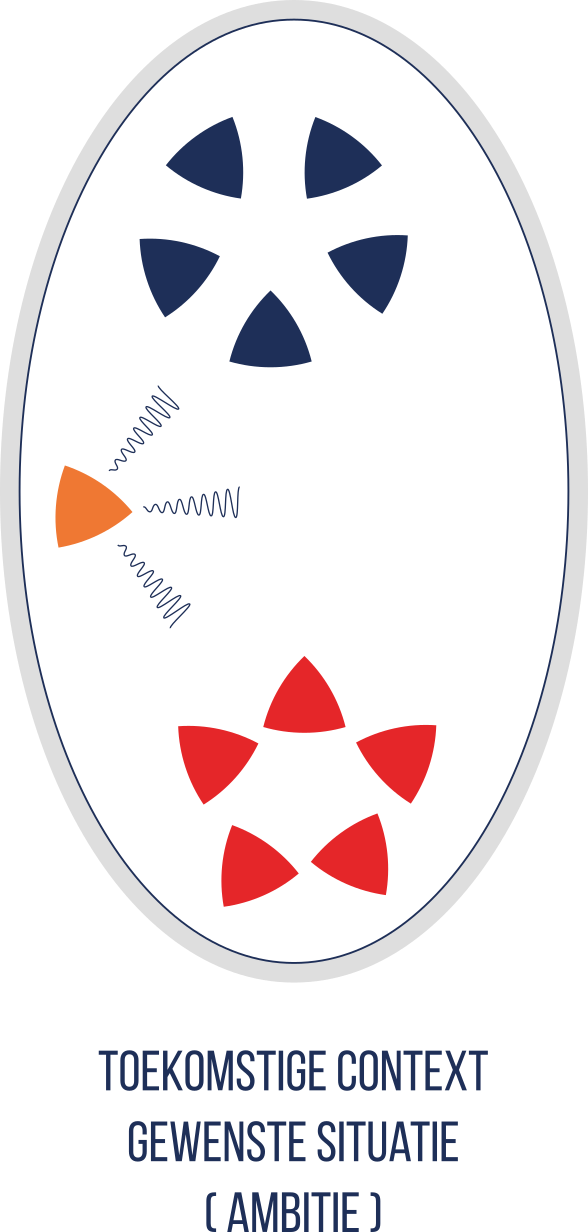
\includegraphics[width=0.2\linewidth]{data/images/20210324-MDI-eieren-beweging-3} 

}

\caption{Abstracte vormgeving van toekomstige context.}\label{fig:eieren-in-beweging-3}
\end{figure}

In een toekomstige context beschrijven we de voorgestelde militaire operationele setting van de beoogde effectbrenger. Hierin beschouwen we de effectbrenger integraal binnen het militaire systeem waarin het na implementatie zal optreden.

Door het opzetten van een toekomstige context krijgen de betrokken actoren een beeld bij de integraliteit en complexiteit van de design opgaaf, wordt gewerkt aan overzicht van relevante lopende initiatieven en onstaat inzicht in de de ontwikkelrichting en meerwaarde van de beoogde effectbrenger. Dit draagt bij aan designkeuzes, organisatie mogelijkheden en indicatoren voor validatie.

Gezamenlijk werken potentiële partners met relevante actoren aan een gemeenschappelijk beeld van de toekomstige setting waarin militaire capaciteiten optreden. Daarin worden ook de gewenste effecten gedefinieerd die het optreden moeten creëeren. De setting met de gewenste effecten maakt de toekomstige context.

\hypertarget{experimentele-context}{%
\subsubsection{experimentele context}\label{experimentele-context}}

\begin{figure}

{\centering 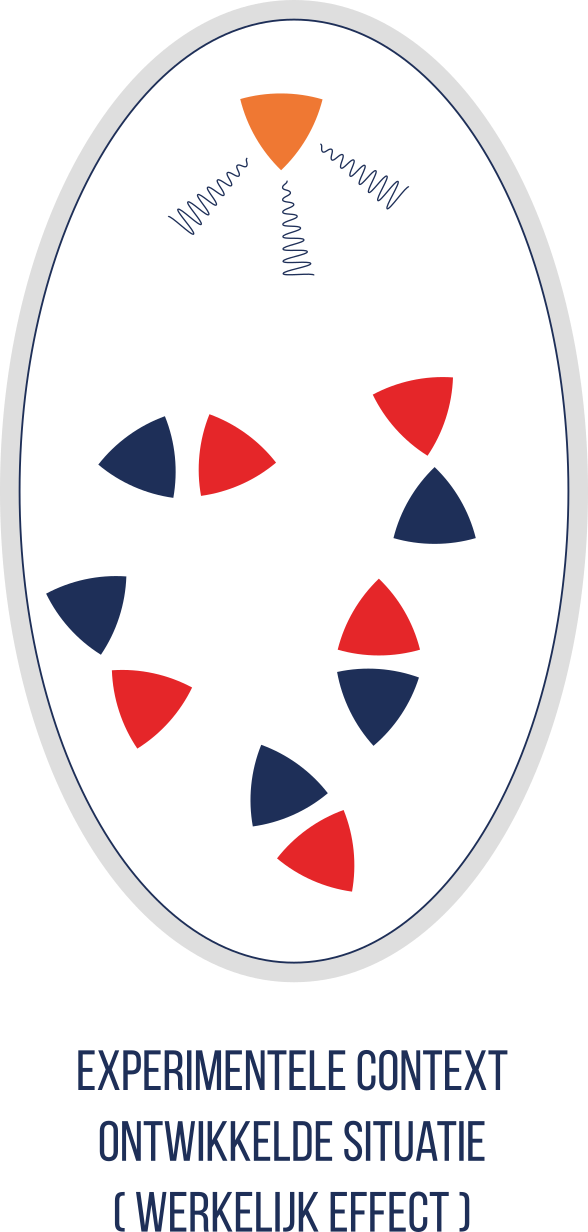
\includegraphics[width=0.2\linewidth]{data/images/20210324-MDI-eieren-beweging-2} 

}

\caption{Abstracte vormgeving van experimentele context.}\label{fig:eieren-in-beweging-2}
\end{figure}

In een experimentele context ontwikkelen en valideren de partners de beoogde effectbrenger. Militaire experimenten kunnen zelden plaatsvinden in een laboratorium of operationele realiteit. Zo realistisch mogelijk wordt de operationele setting van een ontwikkelde effectbrenger nagebootst.

Door het opzetten van een gecontroleerde setting kan de ontwikkelde effectbrenger worden beproefd en kunnen de werkelijke reacties van de omgeving worden waargenomen. De mate van controle is onder andere afhankelijk van het technical readiness level (TRL) van middelen, de maturiteit van de effectbrenger en vigerende wet- en regelgeving. Ook de wijze van meten en valideren beinvloed de gewenste setting van het experiment.

Omdat we het traject zoveel mogelijk in samenhang en tempo doorlopen, starten we zo vroeg mogelijk met het opzetten en vaststellen van de experimentele context. Samen met interne en externe partners, het kenniscentrum en operationele eenheden creëeren we een gecontroleerde operationele omgeving met een eenheid in training, oefening of bij inzet.

\hypertarget{organisatorische-context}{%
\subsection{organisatorische context}\label{organisatorische-context}}

De organisatorische context is de setting van relevante en betrokken actoren en factoren die een relatie hebben of kunnen krijgen met het innovatie traject. Het zijn mensen, manieren en middelen die randvoorwaardelijk zijn voor het succesvol doorlopen van een innovatie traject.

De setting van actoren en factoren brengen we in kaart en de dynamiek verstaan we door de onderlinge relaties en verbindingen te leggen. Het resultaat is een weergave van het multi-actornetwerk wat ondersteund bij het doen van interventies en daarmee beinvloeden van de context.

\hypertarget{factoren}{%
\subsubsection{factoren}\label{factoren}}

Factoren zijn materiële en immateriële zaken zoals feiten, objecten, projecten, systemen, procedures, mechanisme of materieel. De relevantie factoren van invloed op het innovatietraject kunnen vanuit verschillende perspectieven worden beschouwd. Vaak terugkerende perspectieven zijn niveau, domein, vakgebied, projecten/programma's, doctrine en beleid.

Met niveau onderscheiden we het politiek strategisch, militair strategisch, militair operationeel en militair tactisch niveau. Waar nodig kan beleid, bestuur en uitvoeringsniveaus worden onderscheiden.

Binnen de militaire context kent de domeinen, maritiem, land, air, space en cyber. Vakgebieden zijn talrijk zowel binnen de militaire, civiele en academische context. Projecten of programma's worden toegepast op materiële vernieuwing of -vervanging, reorganisatie en kennis- en innovatie. Tot slot worden continue doctrine publicaties aangepast via de NATO en Nederlandse kennsi- en expertisecentra en beleid gecreëerd op de ministeries.

Bronnen voor het identificeren en selecteren van de relevante factoren van invloed zijn ondermeer:
- Defensienota 2018 Invasteren in onze mensen, slagkracht en zichtbaarheid
- Defensie Innovatiestrategie Samen sneller innoveren
- Defensievisie 2035 Vechten voor een veilige toekomst
- Strategische Kennis- en Innovatieagenda 2021-2025
- CDS Aanwijzing A-700 Gereedstelling
- CLAS Toekomstvisie Veiligheid is vooruitzien
- CLAS Operationeel kader voor het landoptreden (OKL)
- CLAS nota Marsrichting, marsroutes en MTO's
- Nederlandse Defensie doctrine
- Doctrine publicatie 3.2 Landoperaties
- Defensie kennis en innovatieplan
- Defensie investeringsplan

\hypertarget{actoren}{%
\subsubsection{actoren}\label{actoren}}

Actoren zijn handelende subjecten zoals individuen, groepen, communities, eenheden, afdelingen, organisatiedelen, bedrijven, instellingen en samenwerkverbanden. In de meeste gevallen spreken we binnen de organisatorische context over organisaties, eenheden en de functionaris die deze vertegenwoordigd.

De relevante actoren van invloed hebben een wederzijdse afhankelijkheid met elkaar en het innovatietraject. Zij proberen elkaar te beinvloeden. ``De pogingen die de actor onderneemt zijn interventies. Een interventie kan van alles inhouden, zoals een regel, mededeling, geld beschikking, informatie, dreiging, verbod, enzovoort.'' (\protect\hyperlink{ref-bruijn2017management}{Bruijn \& Heuvelhof, 2017, p. 16}). Interventies kunnen daarmee factoren zijn die invloed hebben op het innovatietraject.

Dit dynamisch geheel van wederzijds afhankelijke actoren, die interventies plegen, onderlinge variëteit kennen en zich relatief gesloten kunnen opstellen noemt Bruijn \& Heuvelhof (\protect\hyperlink{ref-bruijn2017management}{2017}) een multi-actornetwerk. Dit netwerk kan verbeeld worden in verschillende lagen. Voor de organisatorische context van innovatietrajecten is het onderscheid in een strategische-, management- en uitvoerende laag behulpzaam.

\hypertarget{relaties}{%
\subsubsection{relaties}\label{relaties}}

\begin{figure}

{\centering 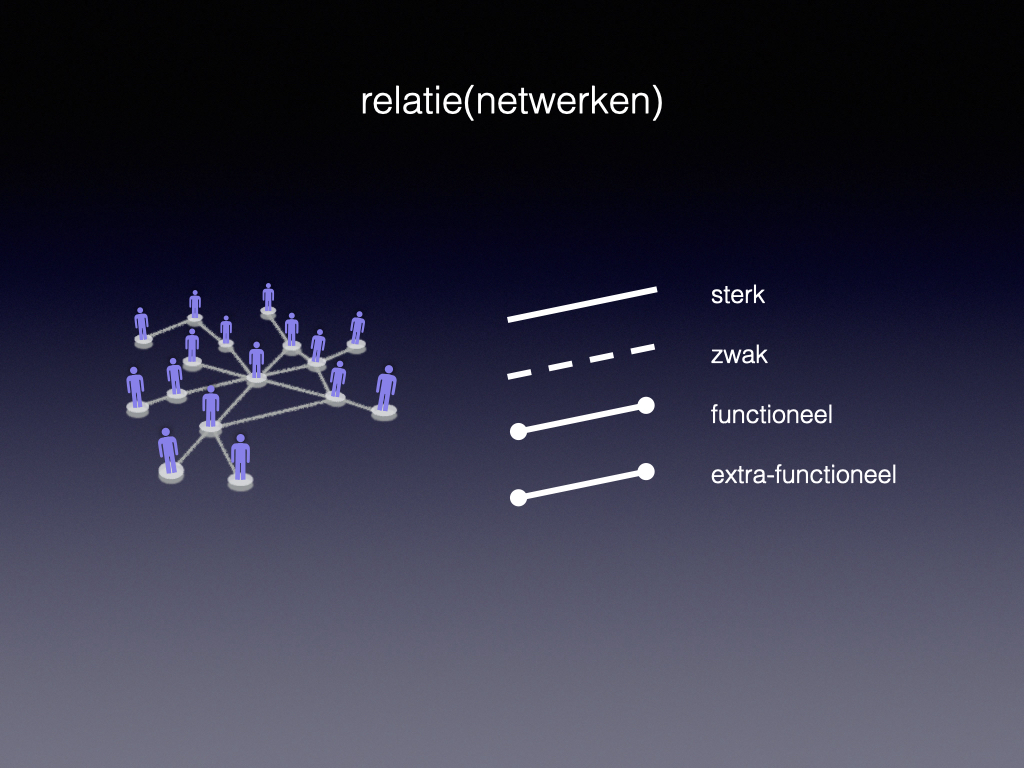
\includegraphics[width=0.6\linewidth]{data/images/presentatie-netwerk9} 

}

\caption{Eigenschappen relaties in multi-actornetwerk}\label{fig:relaties}
\end{figure}

Een netwerkstructuur of multi-actornetwerk is te beschouwen als een verzameling actoren en factoren (nodes) die gedragingen en informatie uitwisselen door tijdelijke relaties (edges) aan te gaan. In een organisatorische context hebben de relevante actoren en factoren onderlinge afhankelijkheden en relaties. Deze relaties kenmerken zich als sterk (intensief gebruik) of zwak (incidenteel gebruik) en als functioneel (de actor kan haar kerntaken niet uitvoeren zonder dit type relatie) of extra-functioneel (handig voor `toevallige' informatie of te toekomst) (\protect\hyperlink{ref-bruijn2017management}{Bruijn \& Heuvelhof, 2017}).

Een specifieke groep actoren die zich verbind op een doel (gemeenschappelijk resultaat) noemen we een collectief. Zo'n collectief ontwikkelt eigen belangen, standpunten, gewenste resultaten en daarmee eigen gedrag. Dit gedrag zorgt voor een nieuwe dynamiek binnen het collectief en vanuit het collectief richting de omgeving.

Geen relatie heeft een permanente status maar ze vertonen op abstract niveau langere tijd gelijkenis. Zeker organisatorische actoren kennen fluïde of kortstondige relaties. Individuele professionals gaan vaak een meer stabiele relatie aan die verder reikt dan een specifiek resultaat of doel. De structuur die hieruit onstaat wordt het relatienetwerk genoemd.

\hypertarget{wicked-problems}{%
\section{wicked problems}\label{wicked-problems}}

In het ontwikkelen van een innovatievraagstuk beschouwen wij deze als een ongetemd probleem in een complexe context. Deze paragraaf \ref{wicked-problems} geeft een korte inleiding en achtergrond bij dit soort problemen.

\textbf{inleiding}

Wanneer potentiele samenwerkende partners verschillende oorzaken of invalshoeken zien voor een probleem spreken we van een ongetemd probleem of \emph{wicked-problem}. Deze ongetemde problemen komen voor in alle lagen, sectoren en gebieden van organisaties en maatschappijen. Ongetemde problemen zijn niet zomaar opgelost en kennen geen afzonderlijke probleemeigenaar of centrale verantwoordelijke. Het `vacuüm' van centrale verantwoordelijke wordt steeds vaker opgevuld door een alliantie van diverse organisaties. Deze allianties zijn van tijdelijke aard en hebben een horinzontale machtsrelatie. In de praktijk creëren deze allianties verrassende oplossingen voor ongetemde problemen.

\textbf{aanpak ongetemde problemen}

Er is geen pasklaar antwoord of eenduidig proces om ongetemde problemen met een alliantie aan te pakken. Wel bestaan er succesvolle voorbeelden met terugkerende activiteiten. De Military Design \& Innovation aanpak is deels geinspireerd door voorbeelden van innovatieve cooperaties en gemeentelijke- en provinciale overheden.

Een aanpak begint met het exploreren van de context en actoren, centraal stellen van (organisatorische) behoeften, belangen, waarden en plichten, en het organiseren in netwerken of ketens. Vervolgens leren de relevante partijen door samen te werken aan oplossingsrichtingen en deze met experimente in de praktijk te brengen. Deze aanpak van exploreren, articuleren en experimenteren passen we toe in Military Design \& Innovation.

\textbf{aanpak in militaire context}

Bij het exploreren van het vraagstuk en de actoren bevinden we ons op onbekend terrein. Aan de hand van succes-indicatoren, canvassen en ambities brengen we in werksessies de context, bestaande initiatieven en stakeholders in kaart, zoals een ontdekkingsreiziger een kaart intekent en daarbij navigeert op bekende referentiepunten met kompas en sextant.

Het resultaat zijn een gearticuleerd probleem, probleemcontext en vraag waarmee potentiele partijen worden benaderd. Partijen willen deelnemen vanwege hun belangen, waarden, interesse of machtspositie en worden geselecteerd als zij een effectieve bijdrage kunnen leveren aan de oplossing(srichting). Afhankelijk van de abstracte of concrete beschrijving van het vraagstuk vinden meerdere iteraties plaats om de vragen en mogelijke oplossingen helder te krijgen.

Een consistente vraagarticulatie slaat een brug tussen de probleem context en ambitie, opdrachtgever en -nemer en idee en implementatie. Het militairy design framework ondersteund de samenwerkende partijen bij het creëren van een consistent geframde en gearticuleerde vraag.

\hypertarget{how-to-design}{%
\chapter{How to design}\label{how-to-design}}

De Landmacht is een uitvoerende organisatie die door de Nederlandse regering of civiele autoriteiten wordt ingezet bij confliten, rampen en crisissituaties. Daardoor komen operationele Landmachteenheden in situaties die uitzonderlijk zijn. De kernprocessen van de Landmacht zijn gericht op het gereedstellen voor inzet onder verzwaarde omstandigheden.

Parallel aan gereedstelling loopt de `modernisering van CLAS' in de waterval aanpak; omgevingsanalyse, doctrine ontwikkeling, concept en plan ontwikkeling, financiering van nieuwe plannen, aanschaf en instroom materieel, en reorganiseren operationele eenheid. De bestaande Landmacht organisatie is in een continue ontwikkel modus vanuit deze volgordelijke aanpak. De processen zijn echter ingericht op instandhouding en langtermijn plannen. Er is daarom behoefte aan nieuwe manieren om innovatie bij de Landmacht integraal met externe partijen uit te voeren in het tempo van de markt.

Verregaande samenwerking met externe partijen vraagt om interconnectiviteit op elkaars processen. Naast gemeenschappelijke denkmodelen (hoofdstuk \ref{how-to-think}) zijn ook gemeenschappelijke ontwerpprocessen nodig. In dit hoofdstuk beschrijven we de design activiteiten en technieken die bijdragen aan het gemeenschappelijk ontwerpen en verbeelden van toekomstige militaire capabilities.

\hypertarget{design-vaardigheden}{%
\section{Design vaardigheden}\label{design-vaardigheden}}

Military Design \& Innovation is voornamelijk een actieve aanpak in dialoog met en over mensen, middelen en manieren. De aanpak bestaat uit een raamwerk (framework) en een activiteiten pallet. De activiteiten leiden tot de verbeelding en creatie van effectbrengers. De basis van deze activiteiten zijn de drie vaardigheden lokaliseren (localize), bevragen (question) en openstellen (open up) (\protect\hyperlink{ref-sennett_craftsman_2008}{Sennett, 2008}).

\textbf{localize}
Lokaliseren gaat over het oog hebben voor details en de capaciteit om de belangrijke aspecten van iets vast te stellen. Een belangrijk begrip hierin is \emph{problem finding} oftewel het ontdekken van de huidige en toekomstige dreigingen, \emph{capability gaps}, en \emph{short falls}. Dit kan worden uitgebeeld in de probleem context. Wanneer de relevante probleem context is geduid kunnen de betrokken professionals werken aan de (door)ontwikkeling van effectbrengers in die context.

\textbf{questions}
Bevragen gaat over het (vragend) onderzoeken van het probleem, de probleem context en betrokken actoren. Een belangrijk begrip hierin is \emph{dwelling} of exploreren. De betrokken professionals verkennen de \emph{problem space} en allerlei mogelijke probleem definities en oplossingsrichtingen. Wanneer de probleem context is verdiept kunnen de betrokken professionals vragen articuleren voor het gericht vinden van relevante (externe) partners.

\textbf{open up}
Openstellen gaat over de betrokken professionals die vrijkomen uit de specifieke context en geeigende oplossingsrichtingen. Een belangrijk begrip hierin is intuitie, het ervaren voorbij de vijf zintuigen en analystiche redeneringen. Door los te komen van de `waan van de dag', focus te brengen op de \emph{problem space}, en te luisteren naar de subtiele gewaarwording komen de betrokken professionals in een flow waarin nieuwe verbanden, kansen en oplossingen aandienen. Wanneer het probleem, de probleem context en de oplossingsrichting is geduid kunnen de betrokken professionals werken aan het vervolg van het traject.

\hypertarget{military-design-innovation-framework}{%
\section{Military Design \& Innovation framework}\label{military-design-innovation-framework}}

Het Military Design \& Innovation framework visualiseert de samenhang van effectbrengers, contexten en ontwikkelproces. Het framework biedt houvast tijdens het ontwerpen, ontwikkelen, experimenteren en samenwerken aan een beoogde effectbrenger in de toekomstige context. Het framework modeleert in één figuur (\ref{fig:design-model}) de ontwikkeling van een effectbrenger, oftewel het traject van idee tot en met valideren in een abstracte visualisatie.

\begin{figure}

{\centering 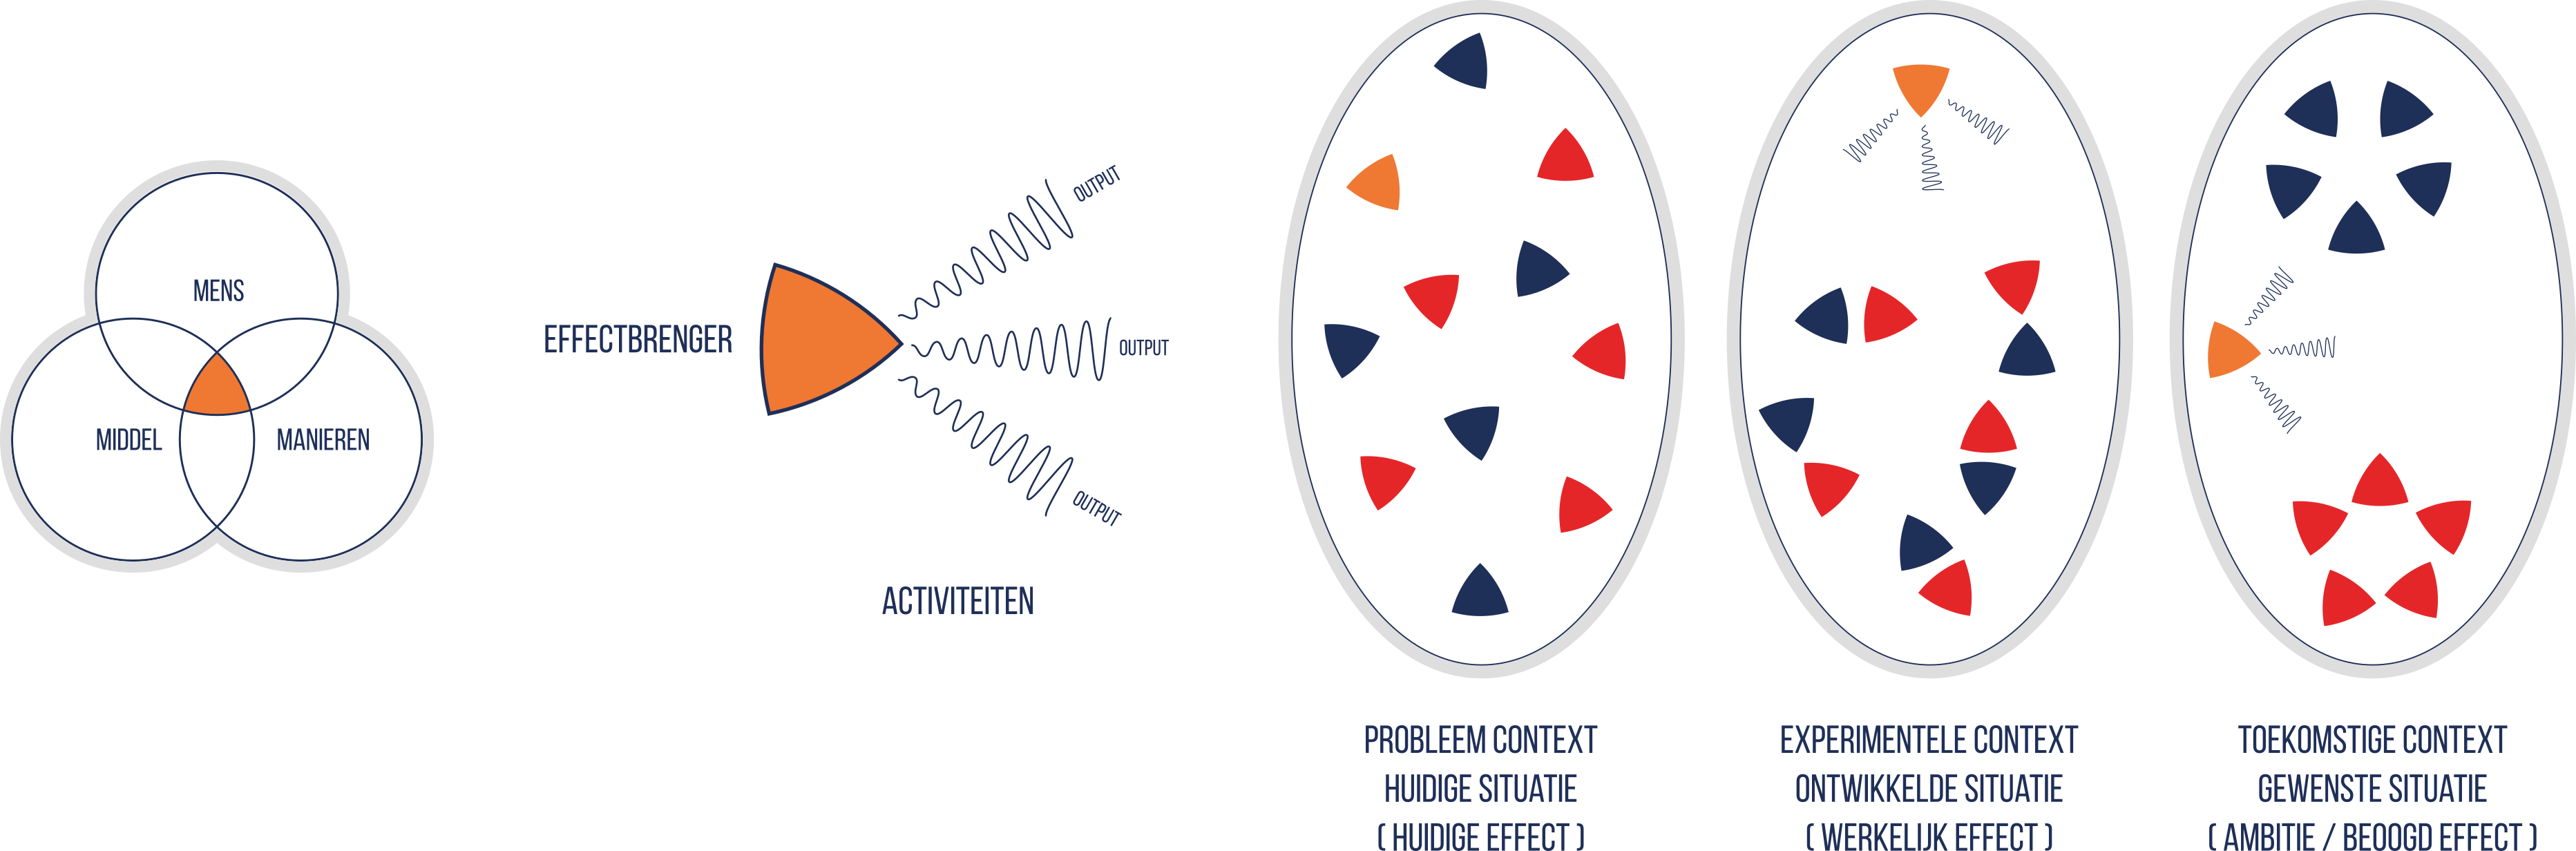
\includegraphics[width=0.8\linewidth]{data/images/20210324-MDI-design-model} 

}

\caption{Military Design \& Innovation framework.}\label{fig:design-model}
\end{figure}

Gezamenlijk creeert een groep professionals inzicht in de mogelijkheden van de markt voor de --toekomstige-- uitdagingen in het landoptreden. Daarin onderkennen we twee bewegingen, vanuit de toekomstige context (forecasting) of vanuit de huidige context (backcasting).
Forecasting gaat van links naar rechts. Dat wil zeggen, door het maken van nieuwe combinaties van mens, manieren en middel ontstaan gemoderniseerde effectbrengers. Met hun activiteiten dragen zij bij aan vernieuwde effecten in een toekomstige context.
Backcasting gaat van rechts naar links. Dat wil zeggen, vanuit ambities en operationele behoeften worden de gewenste effecten, output en activiteit inzichtelijk. Hiermee wordt de beoogde effectbrenger geschetst. Verschillende variaties van de beoogde effectbrenger worden ontwikkeld door het combineren van mensen, manieren en middelen.

In een traject stellen we de hypothese dat een gemoderniseerde effectbrenger bijdraagt aan een gewenst effect in een toekomstige context. Tijdens de experimenten worden gemoderniseerde effectbrengers ingebracht in een afgebakende, gecontroleerde situatie. In deze experimentele context worden de prestaties en effecten gemeten.

\hypertarget{activiteiten-pallet}{%
\section{activiteiten pallet}\label{activiteiten-pallet}}

\begin{figure}

{\centering 
\includegraphics[width=0.85\linewidth]{data/images/20210401-MDI-activiteiten-pallet-1} 

}

\caption{Pallet aan activiteiten binnen Military Design \& Innovatie.}\label{fig:unnamed-chunk-7}
\end{figure}

Om ambities en ideëen te brengen naar implementatie moeten veel activiteiten worden ingezet. Omdat we een idee binnen Military Design \& Innovation benaderen als een ongetemd probleem is er geen uitgestippeld pad maar ligt er een ontdekkingstocht in het verschiet. Om deze tocht te ondernemen moeten we actief worden. Vier activiteiten komen met regelmaat terug in het traject. Tijdens en na de acties reflecteren we op de ondernomen stappen. Wat kunnen de volgende stappen zijn? Welke richting moeten deze stappen opgaan? De reflectie creeert inzicht en overzicht bij de betrokken professionals op hun handelingsperspectieven in het traject.

In deze paragraaf worden de activiteiten van het huidige pallet toegelicht zodat ze worden begrepen. Het doorgronden van de activiteiten vindt plaats in de praktijk. Daarom is praktische uitvoering onder begeleiding belangrijker dan theoretisch bestuderen of werken volgens het boekje.

\hypertarget{idee-generatie}{%
\subsection{idee generatie}\label{idee-generatie}}

\begin{figure}

{\centering 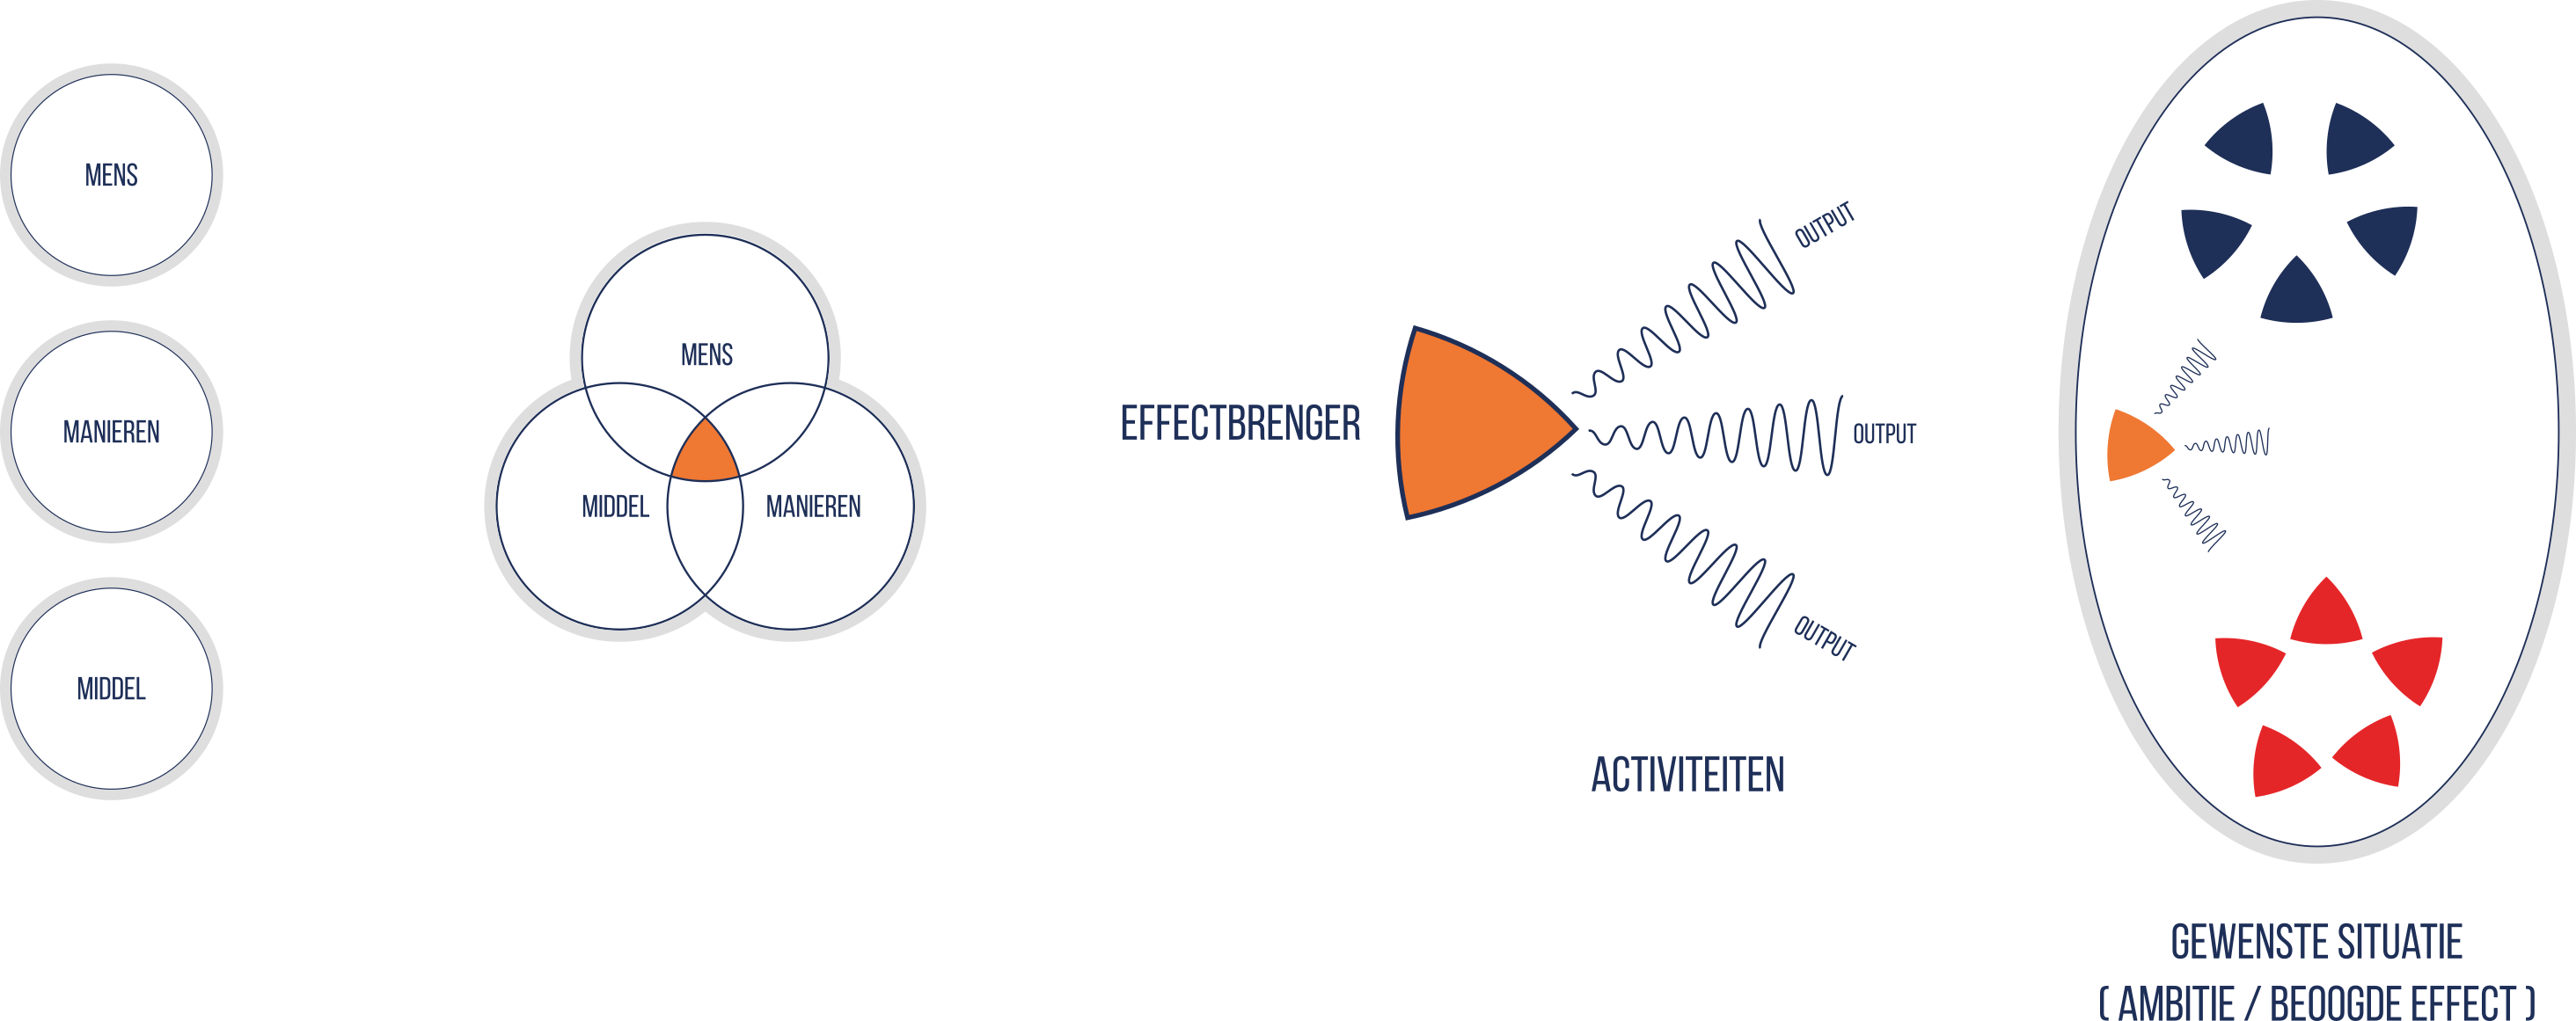
\includegraphics[width=0.9\linewidth]{data/images/20210401-MDI-ideegeneratie} 

}

\caption{ }\label{fig:unnamed-chunk-8}
\end{figure}

In een forecasting komt een kenniswerker of collega van een parate eenheid met een idee wat een verbetering beloofd op de directe taakstelling, werkomgeving of een specifiek vakgebied. Het idee is meestal onvolledig of mist voldoende houvast om direct door te pakken, maar het idee geeft veel informatie over latente vraagstukken, problemen en kansen in een specifieke context. Het is daarom belangrijk om goed te luisteren naar de `binnenlopende ideëen' en deze uit te werken tot een eerste concept. Als ondersteunende tool is hiervoor het canvas `idee generatie 'ontwikkeld. Het stellen van verdiepingsvragen en de 'socratische dialoog' zijn gesprekstechnieken die daarin ondersteunend zijn. De idee-inbrenger beschrijft de beoogde effectbrenger en de toekomstige context kort en bondig zodat dit als idee of design-concept overdraagbaar is.

De centrale deelvragen in deze activiteit zijn:

\begin{enumerate}
\def\labelenumi{\arabic{enumi}.}
\tightlist
\item
  Wat is het idee?
\item
  Wat is er tot nu toe gedaan voor dit idee?
\item
  Wat heb je nodig om dit idee te realiseren?
\item
  Welke stakehodlers of actoren identificeer je?
\end{enumerate}

In een backcasting worden ideëen gegenereerd vanuit ambitie. Het Ministerie van Defensie schetst toekomstscenario's en formuleert ambities en inrichtingsprincipes. De Koninklijke Landmacht beschrijft een visie en ontwikkellijnen. Kennisadviseurs, kenniswerkers en subject matter experts (sme's) programmeren daarbinnen ambities, operationele behoeften en gewenste effecten. In een backcasting worden de operationele behoeften, gewenste effecten, technologische ontwikkelingen en briliante inventies samengebracht. Samen met externe partijen genereren we ideëen voor mogelijke effectbrengers. Voor idee generatie in backcasting wordt de `continue dialoog' gevoerd in een aantal werksessies (zie paragraaf \ref{continue-dialoog}).

\href{data/images/20200116-CDE-canvassen-ideegeneratie.png}{Canvas idee generatie}

\hypertarget{vraag-articulatie}{%
\subsection{vraag articulatie}\label{vraag-articulatie}}

\begin{figure}

{\centering 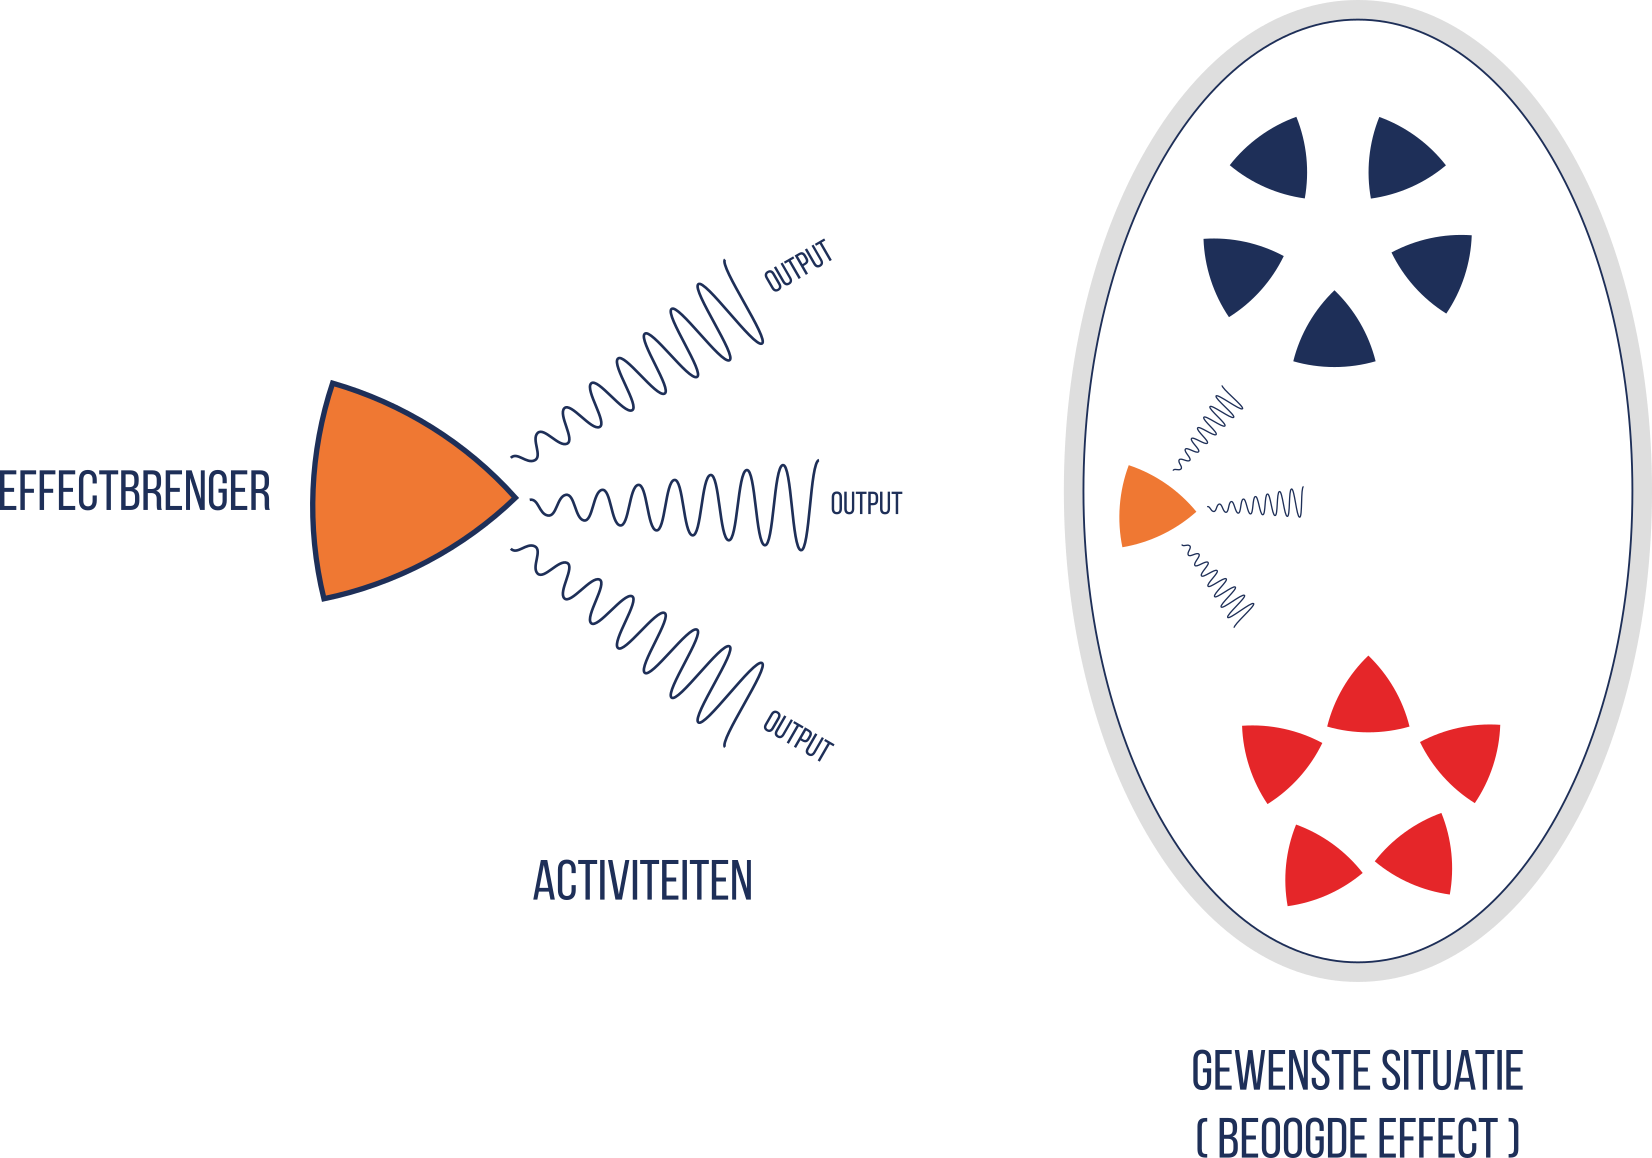
\includegraphics[width=450pt]{data/images/20210324-MDI-effectbrenger-ei} 

}

\caption{ }\label{fig:unnamed-chunk-9}
\end{figure}

Bij het ontwikkelen en experimenteren van nieuwe effectbrengers betrekken we het innovatieve vermogen wat buiten de Defensie organisatie ligt. Om de juiste partners te vinden is het belangrijk een duidelijke vraag te stellen. Dat begint met het spreken van eenzelfde taal en het begrijpen van je eigen behoefte. De ervaringen die we daarin maakte zijn verwerkt in het canvas `vraag articulatie'. Aan de hand van het canvas weet de trajectbegeleider, kenniswerker en ervaringsdeskundige een compleet beeld te schetsen van de probleemcontext, probleem en de uitdaging voor de organisatie. Vanuit dat beeld formuleren we samen met interne specialisten de markt-, onderzoek- of ontwerpvragen.

De centrale deelvragen in deze activiteit zijn:

\begin{enumerate}
\def\labelenumi{\arabic{enumi}.}
\tightlist
\item
  Wat is de operationele context?
\item
  Wat is het probleem of kans of risico (in de context)?
\item
  Wat is de uitdaging (voor de organisatie)?
\item
  Wat is je oplossingsrichting?
\item
  Wat is je vraag?
\end{enumerate}

In een forecasting leiden deze vragen tot een schets van de huidige context met een specifiek probleem en een beoogde effectbrenger. Ook wordt duidelijk waarom dit idee niet door de eigen organisatie of eenheid is op te lossen.

In een backcasting resulteren deze vragen in een geschetste toekomstige context (\ref{toekomstige-context}) waarin een effectbrenger zal acteren.

Vraagarticulatie leidt tot een duidelijker beeld van de beoogde effectbrenger en de positie die deze effectbrenger heeft --of kan krijgen-- in de bestaande organisatie.

\href{data/images/20200116-CDE-canvassen-vraagarticulatie.png}{Canvas vraag articulatie}

\hypertarget{traject-organiseren}{%
\subsection{traject organiseren}\label{traject-organiseren}}

\begin{figure}

{\centering 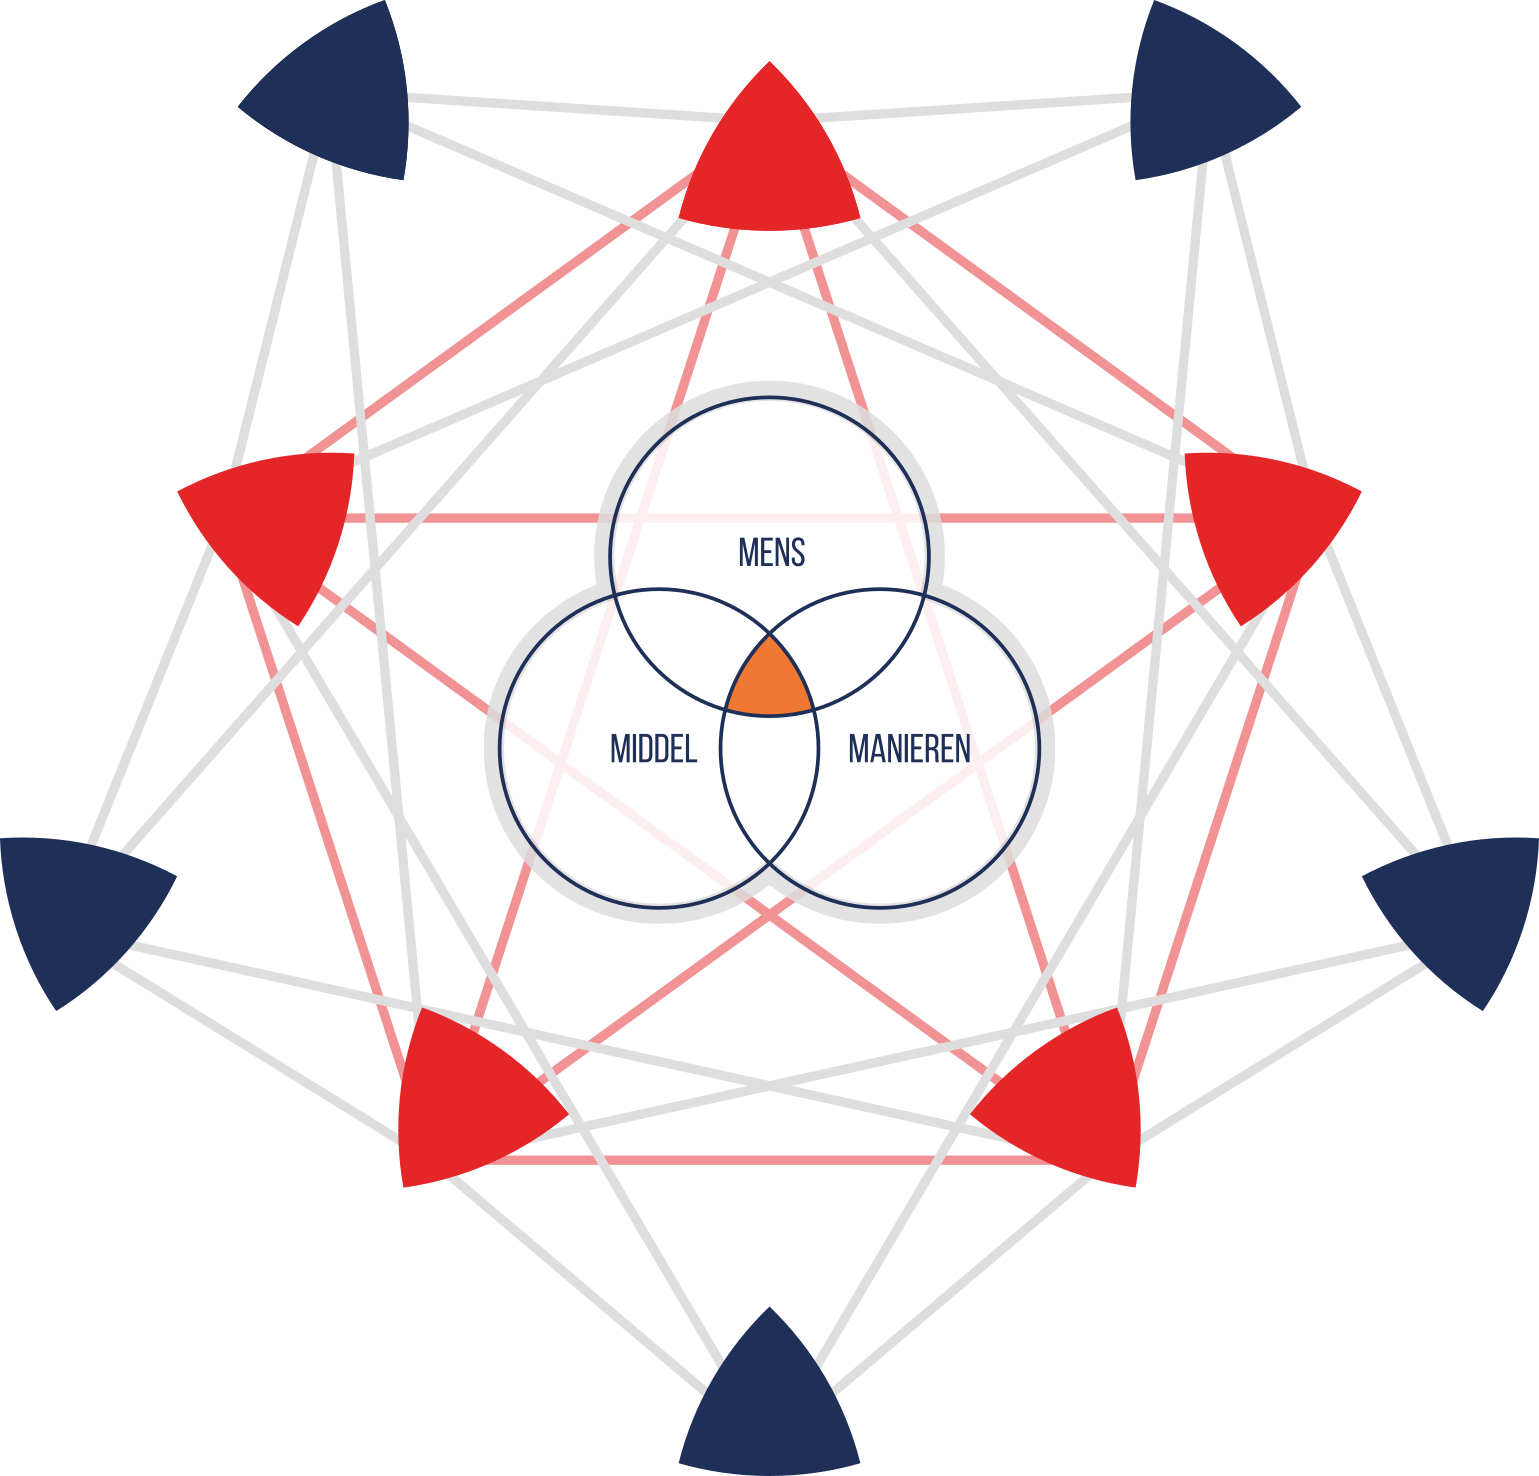
\includegraphics[width=350pt]{data/images/20210401-MDI-trajectorganiseren} 

}

\caption{ }\label{fig:unnamed-chunk-10}
\end{figure}

Rondom een ambitie of idee is een netwerk nodig wat dit idee gaat realiseren. Een tijdelijk netwerk met een eigenaar, projectleider, inkoper, producent, dienstverlener en/of kenniswerker, maar ook een experimenteeromgeving, middelen en specifieke kennis en vaardigheden. Deze actoren en factoren worden samengebracht in een projectorganisatie. Zij organiseren samen alle noodzakelijke activiteiten om het idee te ontwikkelen, experimenteren en valideren.

De ervaringen om een organisatie op te zetten zijn verwerk in het canvas `traject organiseren'. Aan de hand van het canvas weet de trajectbegeleider, kenniswerker en ervaringsdeskundige een `business-' of `valueproposition' te schetsen waarmee relevante actoren worden benaderd.

De centrale deelvragen in deze activiteit zijn:

\begin{enumerate}
\def\labelenumi{\arabic{enumi}.}
\tightlist
\item
  Wat zijn de benodigde key resources?
\item
  Wat zijn de key activities?
\item
  Wie zijn de key partners?
\item
  Wat zijn de voorziene kosten of investeringen?
\item
  Wat is de impact van het project op verschillende levels, contexten of niveau's?
\item
  Hoe zijn de actoren gepositioneerd in de actorenroos?
\item
  Wat zijn de relevante aspecten voor het experiment en de experimenteeromgeving?
\end{enumerate}

Traject organiseren leidt tot een duidelijker beeld van de relevante actoren, zoals kenniseigenaar, projectleider, probleem-eigenaar, werkgever (i.r.t. bedrijfsveiligheid) en experimenteer-omgeving. In deze activiteit wordt ook de `verwerving en levering' voor het project voorbereid en adviseurs geconsulteerd om te anticiperen op potentiële hindernissen in het vervolgtraject en de implementatie.

\href{data/images/20200116-CDE-canvassen-trajectorganisatie.png}{Canvas traject organisatie}

\hypertarget{verwerving-en-levering}{%
\subsection{verwerving en levering}\label{verwerving-en-levering}}

Om innovatie bij de Landmacht uit te voeren in het tempo van de markt moeten randvoorwaarden worden ingericht die niet beschikbaar zijn in de bestaande organisatie. Dit leidt tot een behoefte aan producten, diensten of partnerschappen. Deze worden voor de duur van het traject verworven door onze dedicated inkopers.

Een inkoopadviseur of inkoper adviseert (en bepaald) de verwervingsstrategie. De betrokkenheid van de inkoper vanaf de start van het traject zorgt voor de snelst mogelijke aanvang van de wettelijke procestijd. Met deze korte lijn krijgen we snelheid en houden we controle in de verwerving en levering. Ook zorgen korte lijnen en nauwe samenwerking met inkoop voor vertrouwen en mogelijkheden om andere dan de meest geeigende inkoopstrategiëen toe te passen.

Voor een betrouwbaar inkoopproces is het noodzakelijk om binnen de wet- en regelgeving te opereren. Tot nu toe bieden de dertien inkoopstrategieën altijd een oplossing voor verwerving. De meest effectieve strategie draagt zorg voor een mogelijke implementatie van het design-concept in de toekomst. Binnen Military Design \& Innovation kiezen we niet voor de korte termijn oplossingen maar selecteren de meest effectieve inkoopstrategie voor het totale beoogde traject.

In tegenstelling tot de meeste inkooptrajecten wordt binnen Military Design \& Innovation het inkopen, leveren en contractmanagement onder directe regie van hetzelfde projectteam uitgevoerd. Ook dit draagt bij aan de voortgang van het traject.

\hypertarget{continue-dialoog}{%
\subsection{continue dialoog}\label{continue-dialoog}}

\begin{figure}

{\centering 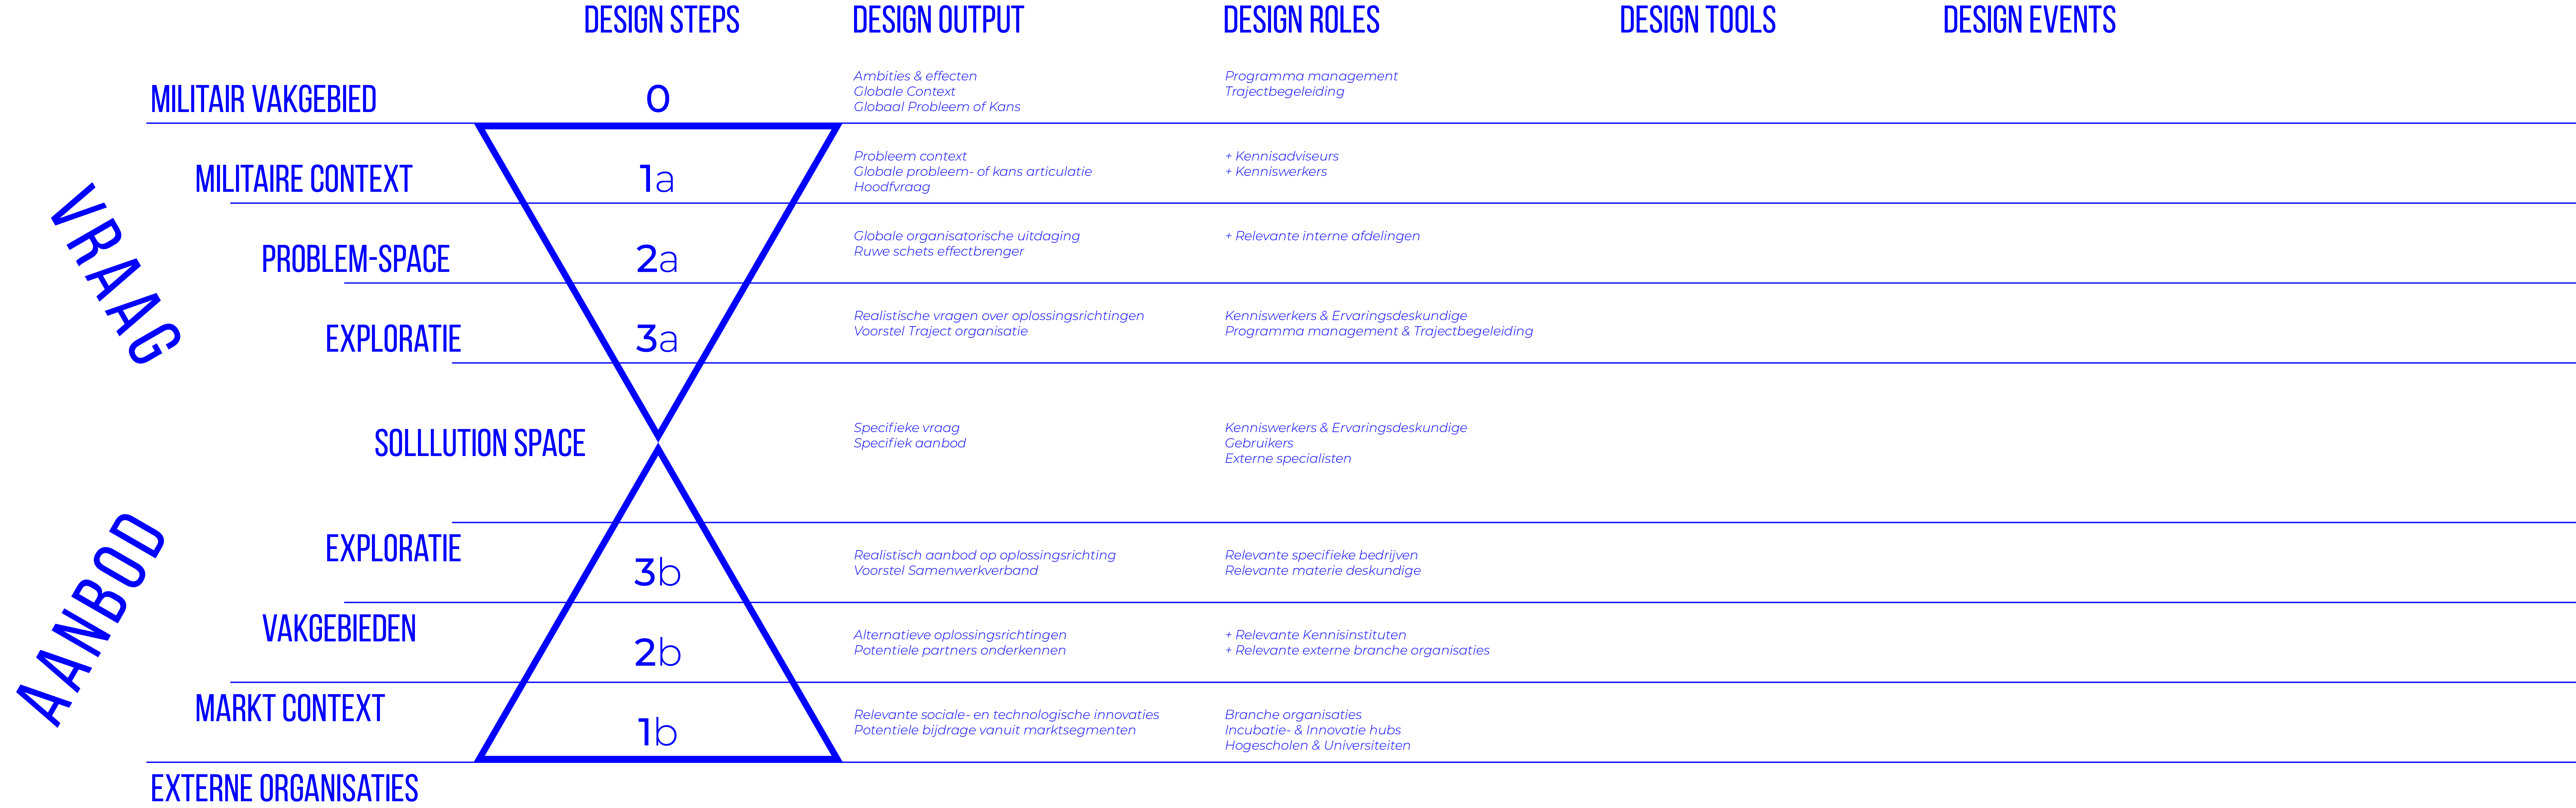
\includegraphics[width=0.6\linewidth]{data/images/20200426-CDE-designproces_vraag-aanbod-exploratie_blauwdruk-v2} 

}

\caption{Eerste schets van het concept vraag-aanbod exploratie zoals toegepast in de dialoog }\label{fig:vraag-aanbod}
\end{figure}

Met de `continue dialoog' worden externe partijen in een vroegtijdig stadium betrokken in een thematisch programma of bij een technisch vraagstuk. De `continue dialoog' kent een aantal stadia waarin het vraagstuk steeds concreter wordt met hulp van de externe partijen. Figuur \ref{fig:vraag-aanbod} visualiseert een dialoog naar vraagarticulatie en aanbodspecificatie. Het toelopen van de lijnen naar het middelpunt suggereert het convergerend werken in een aantal werksessies of stappen naar het punt waarop de vraagarticulatie en aanbodspecificatie elkaar vinden.

Afhankelijk van het vraagstuk en de context worden relevante partijen door SBID-medewerkers gekoppeld aan de dialoog. De verantwoordelijk programma-manager voert de regie in de dialoog en draagt deze in een latere fase over aan de trajectbegeleider.

\hypertarget{how-to-develop}{%
\chapter{How to develop}\label{how-to-develop}}

De Landmacht ontwikkeld en innoveert in een context met een veelheid aan politieke, economische, academische en sociaal-maatschappelijke belangen. Kenmerken van deze organisatorische context zijn de complexiteit van vraagstukken (inhoud), verwevenheid van actoren (relaties) en het ontbreken van formele kaders (macht). Hierin onstaan complexe genetwerkte problemen (\protect\hyperlink{ref-dorst_mixing_2018}{Dorst, 2018}) waar de bureaucratische en hierarchische Defensie organisatie niet altijd effectief en wenselijk kan handelen.

In deze organisatorische context zoekt de Landmacht naar innovaties die over de grenzen van organisaties en vakdisciplines heengaan. Een genetwerkte vraaggerichte aanpak in de organisatorische context moet bestaan naast de hierarchische opdrachtgerichte aanpak in de operationele context van de Landmacht. Dit maakt multi-disciplinair en multi-organisationeel samenwerken uitdagend. Zeker als de actoren in nieuwe, onbekende rollen terrecht komen. Het is dan extra belangrijk om elkaar, de contexten en omstandigheden te begrijpen.

De professionals moeten hierin effectief acteren zodat de belangen voor de Landmacht en het landoptreden geborgd zijn. Verregaande samenwerking met externe partijen vraagt om interconnectiviteit op de verschillende niveaus van elkaars organisatie. Naast gemeenschappelijke denkmodelen (hoofdstuk \ref{how-to-think}) en ontwerpprocessen (hoofdstuk \ref{how-to-design}) zijn ook realisatie vaardigheden en processen nodig. In dit hoofdstuk beschrijven we de enkele relevante actoren en factoren die bijdragen aan het gemeenschappelijk ontwikkelen en realiseren van toekomstige militaire capabilities.

\hypertarget{realisatie-vaardigheden}{%
\section{realisatie vaardigheden}\label{realisatie-vaardigheden}}

Military Design \& Innovation is een aanpak gericht op realisatie samen met de relevante interne\footnote{Met interne actoren worden medewerkers en organisatiedelen van het Ministerie van Defensie.} en externe actoren. De bijhorende strategiën hebben drie kenmerken gemeen die als vaardigheden van de professional terugkomen. Dit zijn verbinden, versnellen en vermarkten.

\textbf{verbinden}
De professional en organisatie zet zich in om de procedures, afdelingen, functionarissen, projecten en programma's met elkaar te verbinden op het specifieke innovatie vraagstuk. Door de contacten in de Directie K\&O en de Defensie organisatie beschikt het multi-disciplinaire team over een groot relatienetwerk en creëeren zij overzicht en inzicht in de innovatie initiatieven die binnen de organisatie spelen.

\textbf{versnellen}
Overheidsorganisaties als het Ministerie van Defensie dient transparant, non-discriminatief en proprotioneel om te gaan met de opgedragen taken en toebedeelde middelen van de maatschappij. De daaruit volgende bureaucratische organisatie draagt zorg voor het hoog houden van de sociaal-maatschappelijke waarden. Soms slaan regels en procedures door of blijken te ontbreken. Dit kan zorgen voor vertragingen bij het innoveren. Vertragingen worden adequaat opgepakt met kennis van de processen, vaardigheid in de handelingsperspectieven en de contacten met verantwoordelijke functionarissen of afdelingen. De Afdeling Innovatie heeft het vertrouwen binnen de organisatie om verantwoord en doelgericht te handelen binnen de staande wet- en regelgeving.

\textbf{vermarkten}
De oplossingen voor de innovatie vraagstukken van de Landmacht liggen bij externe partners zoals MKB, kennisinstituten en start-ups. Samenwerken aan gemeenschappelijke belangen is daarin een belangrijk uitgangspunt. Door de vragen in de Landmacht-organisatie te koppelen aan het oplossingsvermogen van externe partijen ontstaan de military capabilities van de toekomst.

De verbinding tussen professionals creëert daarbij ook toegang tot de juiste afdelingen en functionarissen binnen de organisatie wat bijdraagt aan relatienetwerk vol diversiteit.

\hypertarget{aanpak-van-innovatie}{%
\section{aanpak van innovatie}\label{aanpak-van-innovatie}}

In het Military Design \& Innovation framework zien we de samenhang van effectbrengers, contexten en ontwikkelproces. In het design proces ligt de focus op de effectbrengers en de operationele contexten. Naast het design proces (verbeelden) kent het innovatietraject ook een realisatieproces (maken). In het realisatieproces ligt de focus op de organisatorische contexten, het ontwikkelen, valideren en implementeren van de militaire capability.

In het realisatieproces is het belangrijk om een compleet mogelijk beeld te krijgen op de organisatorische context. Het is vervolgens aan het multi-disciplinaire team om de activiteiten zo te plannen en organiseren dat het innovatie vraagstuk succesvol wordt ontwikkeld, geëxperimenteerd en gevalideerd.

Om dit te bereiken zijn vele strategiëen, organisatorische activiteiten en tactieken toepasbaar op een innovatietraject. De Afdeling Innovatie kiest voor een programmatische aanpak bij het realiseren van innovatie. Military Design \& Innovation ondersteund deze aanpak met het multi-actornetwerk denken \footnote{Een verdere toelichting is beschreven in paragraaf @ref(organisatorische context)}. Deze `thinking tool' is aanvullend op het programma-management van de innovatiethema's en projectmanagement van de innovatieprojecten.

Allereerst een korte beschrijving van de termen traject, project en programma binnen de Afdeling Innovatie.

\textbf{project}
Een project is een afgebakende activiteit met toegewezen resources en vastgelegde (externe) partners om een specifiek capability concept te ontwikkelen, experimenteren en/of valideren.

\textbf{programma}
Een programma is een thematisch ingericht `verzamelgebied' waarvoor we resources en partners zoeken en binden en waarin we verschillende initiatieven (projecten, fieldlabs, NTP's, onderzoeken) optuigen om de Landmacht ambities na te streven.

\textbf{traject}
Een traject is de keten van (proces)activiteiten die relevante spelers doorlopen om een idee of ambitie te brengen tot structurele opname in de staande organisatie (implementatie).

Waar projecten en programma's zijn gericht op het bereiken van een gedefinieerd doel met inzet van mensen en middelen, is een traject een proces om het denken en handelen te richten en ondersteunen.

\hypertarget{netwerk-benadering}{%
\subsection{netwerk benadering}\label{netwerk-benadering}}

De professional bezit enige kennis van netwerkdynamiek om strategisch te acteren en bewust te handelen in de organisatorische context. Binnen Military Design \& Innovation wordt het multi-actornetwerk model gebruikt als thinking tool waarmee de professional effectief gedrag vertoont. In dit model wordt de context beschouwd als een netwerk van relevante actoren en factoren met onderlinge interacties.

\hypertarget{actoren-1}{%
\subsubsection{actoren}\label{actoren-1}}

\begin{figure}

{\centering 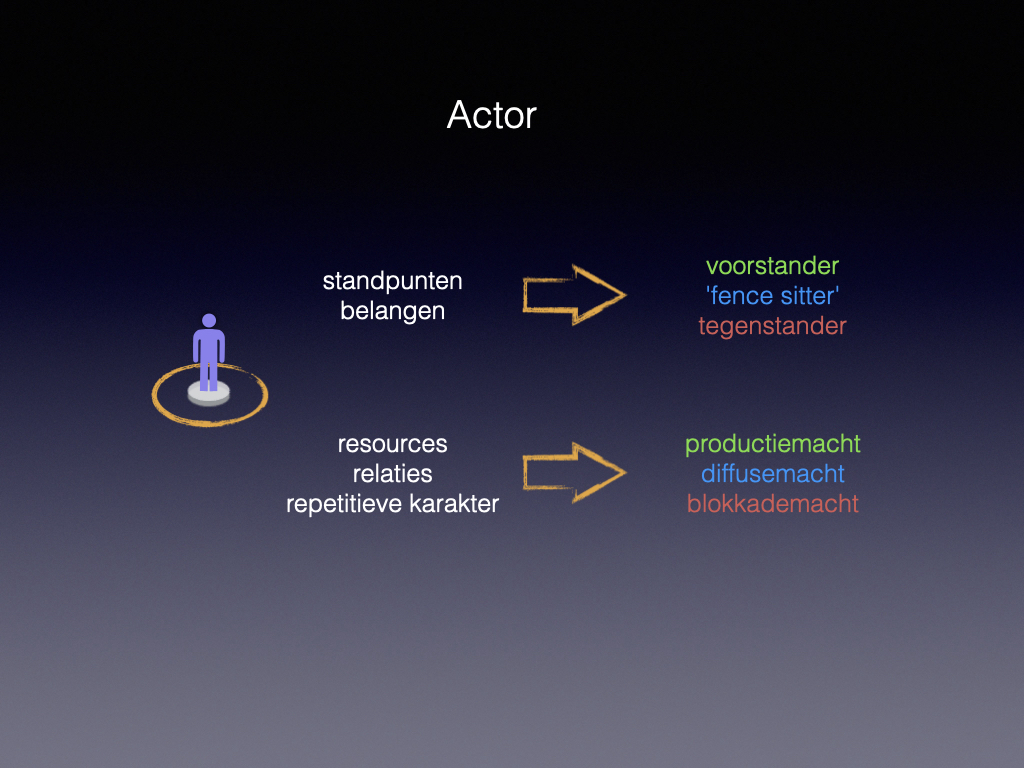
\includegraphics[width=0.6\linewidth]{data/images/presentatie-netwerk7} 

}

\caption{Eigenschappen actor in multi-actornetwerk}\label{fig:actoren}
\end{figure}

De relevante actoren en factoren van invloed op het traject worden zo vroeg als mogelijk betrokken. Daarbij wordt rekening gehouden met hun standpunt en de hun potentiële macht. Deze vormen het gedrag van de actor in de context.

De actoren\footnote{in deze worden ook factoren zoals programma's en projecten bedoelt.} hebben standpunten, belangen, middelen, relaties en een repetitief karakter. Dit maakt dat een actor zich verhoud tot anderen als voorstander, `fence sitter'\footnote{positie is neutraal of er is nog geen keuze gemaakt.} of tegenstander. Een actor is daarbij een productie-, diffuse- of blokkademacht. Op basis van deze aspecten wordt de interactie gezocht met een betreffende actor.

\hypertarget{interactie}{%
\subsubsection{interactie}\label{interactie}}

\begin{figure}

{\centering 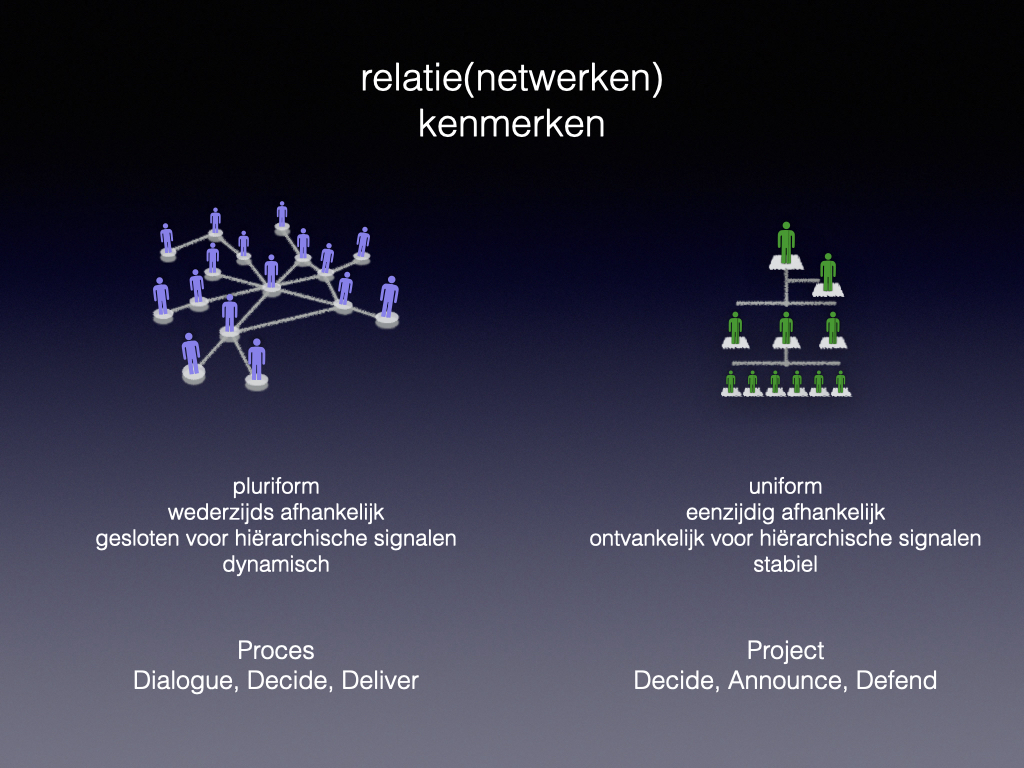
\includegraphics[width=0.6\linewidth]{data/images/presentatie-netwerk10} 

}

\caption{Kenmerken van een verbonden multi-actornetwerk}\label{fig:verbinding}
\end{figure}

Door de setting en gedragspatronen van relevante actoren\footnote{in deze worden ook factoren zoals programma's en projecten bedoelt.} in kaart te brengen en te verbinden met het innovatievraagstuk creëert het multi-disciplinaire team de organisatorische context waarbinnen een specifiek innovatietraject kan worden doorlopen.

Binnen Military Design \& Innovation worden twee soorten netwerken onderscheiden, een multi-actornetwerk en een relatienetwerk. Een actor maakt deel uit van een multi-actornetwerk als zij samen met anderen een patroon van interdependente relaties aangegaan om een gemeenschappelijk resultaat te bereiken. Een actor beschikt over een relatienetwerk als zij een geheel aan relaties met anderen onderhoud. Een actor zit dus in een multi-actornetwerk en beschikt daarbij over een relatienetwerk (\protect\hyperlink{ref-bruijn2017management}{Bruijn \& Heuvelhof, 2017}).

Bijna alle actoren\footnote{in deze worden ook factoren zoals programma's en projecten bedoelt.} in de innovatiecontext van Defensie zijn verbonden in relatienetwerken. Een initiatiefnemer moet de relaties voor een innovatievraagstuk nog wel activeren. Volgens Bruijn \& Heuvelhof (\protect\hyperlink{ref-bruijn2017management}{2017}) kenmerken relaties zich als sterk (intensief gebruik) of zwak (incidenteel gebruik) en als functioneel (de actor kan haar kerntaken niet uitvoeren zonder dit type relatie) of extra-functioneel (handig voor `toevallige' informatie of te toekomst). Voor het multi-actornetwerk op een specifiek vraagstuk worden de relaties `sterk' en `functioneel' gemaakt door het multi-disciplinaire team.

De mate waarin en het tijdstip waarop het multi-disciplinaire team de interactie zoekt met een actor is afhankelijk van veel factoren. Door de interactie te overwegen en plannen ontstaat strategisch gedrag van het team en de omgeving. Dit `spel' gaat vooral over macht en positie en veel minder over de inhoud van het innovatievraagstuk. De professional werkzaam in het innovatielandschap van Defensie moet zich hiervan bewust zijn.

\hypertarget{realisatieproces}{%
\section{realisatieproces}\label{realisatieproces}}

Het ontwerpen en maken van een militaire capability verloopt parallel binnen Military Design \& Innovation. Nadenken over het ontwerp geeft inzichten voor het maken en vice versa. Beide processen versterken elkaar en dragen bij aan het uiteindelijke implementeren van het design concept van de toekomstige militaire capability.

In een traject loodst een multi-disciplinair team het specifieke innovatievraagstuk door een aaneenschakkeling van activiteiten. Hierdoor ontwikkeld het multi-disciplinaire team met partners de beoogde effectbrenger van concept tot een valide militaire capability. Het traject is geen voorgeschreven set aan regels, formules of procedures maar een situationeel en context afhankelijk toepassen van de meest effectieve interactie tussen actoren, activiteiten en technieken om het idee te laten slagen. Het traject is een ontdekkingsreis met één gemeenschappelijk doel, het specifieke idee brengen tot de implementatie van een vernieuwd militair concept in het landoptreden.

De inzichten op het vraagstuk en aansluiting van actoren groeien onvoorspelbaar en in wisselend tempo. Iedere actor brengt nieuwe inzichten op het vraagstuk en vanuit het vraagstuk ontstaat weer behoefte aan andere actoren. Dit is een itteratief of cyclisch proces. Om deze groeicurve en de activiteiten in het traject enigszins overzichtelijk te maken is een fasering aangebracht.

\hypertarget{fasering}{%
\subsection{fasering}\label{fasering}}

\begin{figure}

{\centering 
\includegraphics[width=0.85\linewidth]{data/images/20210401-MDI-activiteiten-pallet-2} 

}

\caption{Fasering van het proces voor Military Design \& Innovatie.}\label{fig:unnamed-chunk-11}
\end{figure}

In het innovatietraject herkennen we drie fasen; het ontwikkelen van een plan, experimenteren met het idee en valideren van de resultaten. Deze fasen moeten leiden tot implementatie waar het multi-disciplinaire team in principe de verantwoordelijkheid overdraagd aan de afdelingen binnen de staande organisatie.

\hypertarget{ontwikkelfase}{%
\subsubsection{ontwikkelfase}\label{ontwikkelfase}}

Tijdens de ontwikkelfase worden ambities verwoord, ideeën gegenereerd, vragen gearticuleerd en het samenwerkverband georganiseerd. Afhankelijk van het vraagstuk kan dit abstract of onduidelijk zijn maar ook specifiek en gedetaileerd. De ontwikkelfase resulteerd in een plan waarin staat wie --in beginsel-- samenwerkt, wat het gemeenschappelijk resultaat is en via welke route het samenwerkverband het gemeenschappelijk resultaat hoopt te bereiken.

\hypertarget{experimenteerfase}{%
\subsubsection{experimenteerfase}\label{experimenteerfase}}

In de experimenteerfase wordt de beoogde effectbrenger (door)ontwikkeld, de experimentele context gecreeerd en het idee getoetst in de ontwikkelde situatie. Afhankelijk van het vraagstuk is de effectbrenger al ontwikkeld of worden prototypen gedurende het experiment in iteraties doorontwikkeld op basis van testresultaten. De experimeteerfase resulteerd in een rapport met de meetwaarden, praktische resultaten en werkelijke effecten van ingebrachte effectbrengers.

\hypertarget{validatiefase}{%
\subsubsection{validatiefase}\label{validatiefase}}

Met de validatie evalueren de samenwerkende partners, de opdrachtgever en relevante subject matter experts de effectbrenger en de resultaten van het experiment op de vooraf gedefinieerde waardenpropositie. Samen wegen zij of de effectbrenger in voldoende maten bijdraagd aan het beoogde effect, gewenste situatie en de toekomstige context. Het resulterende rapport geeft input aan de implementatie van het design concept.

\hypertarget{implementatiefase}{%
\subsubsection{implementatiefase}\label{implementatiefase}}

Voor het opnemen van de vernieuwde capabilities binnen de Krijgsmacht moeten verschillende processen worden opgestart. Hiervoor moet de unieke combinatie van mens, manieren en middelen (beoogde effectbrenger) worden opgespitst in organisatorische wijzigingen (re-organisatie traject), doctrine aanpassingen (doctrine publicatie wijzigingen) en materieelprojecten (projectkaarten in het DLP wijzigen of inbrengen). Het multidisciplinaire team houdt rekening met de initiatie van deze afzonderlijke elementen tijdens het hele traject. Ook bewaakt het multidisciplinaire team de initiatie na rapportage over de bevindingen uit de validatie fase.

\hypertarget{leiderschap}{%
\section{leiderschap}\label{leiderschap}}

Leiderschap is het beinlvoeden van anderen zodat jouw rechten, plichten, belangen, wensen en behoeften worden nagestreefd. Iedere organisatie, organisatiedeel en professional past leiderschap toe.

Iedere fase kent een specifieke dynamiek. De ontwikkelfase heeft een verkennend karakter, de context wordt getekend en een probleem wordt gezocht en gedefinieerd. De experimenteerfase heeft een exploratief karakter, oplossingen worden gecreëerd en getest en de context wordt uitgedaagd. De validatiefase heeft een onderzoekend karakter, de oplossing en de resulterende context worden gestaafd aan het beoogde toekomstig militair optreden. De verschillende fasen kennen daarbij ook specifieke wetten en standaarden.

De kunst is in deze dynamiek de belangen samen te brengen tot een gemeeschappelijk resultaat of doel. Daarvoor vertonen actoren strategisch, tactisch en uitvoerend gedrag. Ze nemen in de verschillende fasen een rol aan om het eigen- en gemeenschappelijk belang na te streven.

\hypertarget{defensie-leiderschapskompas}{%
\subsection{Defensie leiderschapskompas}\label{defensie-leiderschapskompas}}

\begin{figure}

{\centering 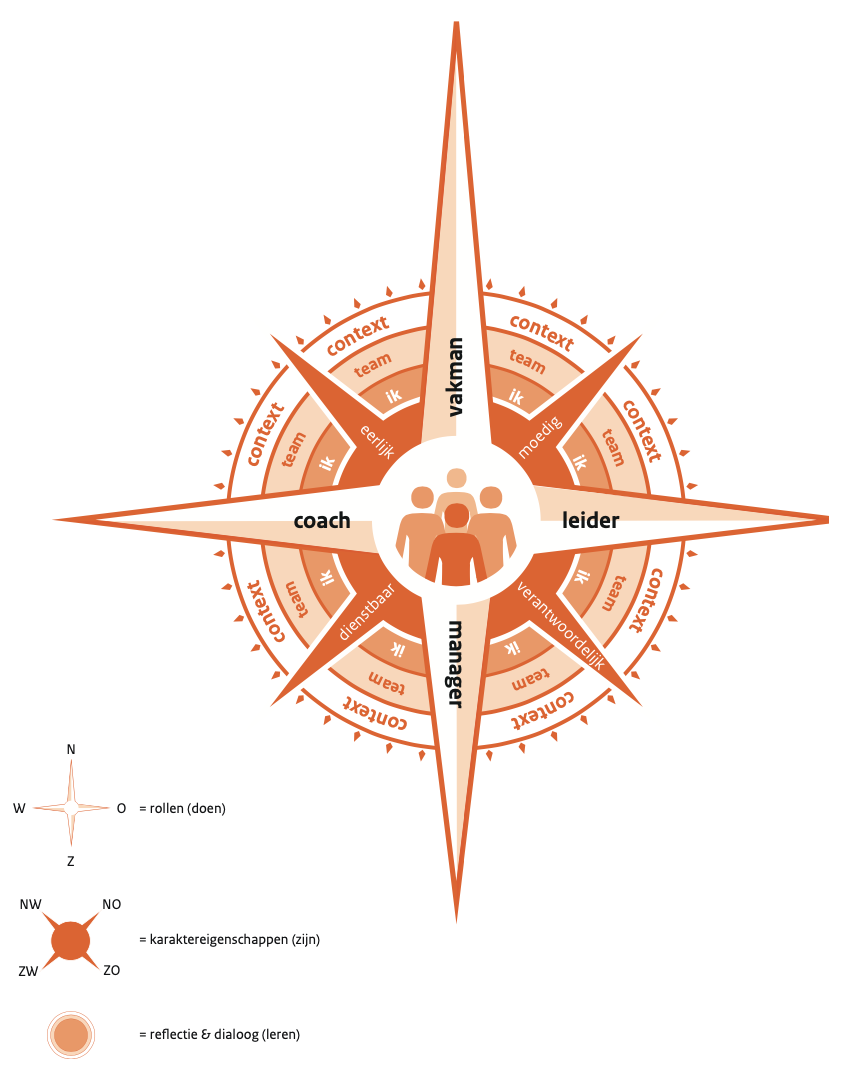
\includegraphics[width=0.7\linewidth]{data/images/leiderschapskompas} 

}

\caption{Leiderschapskompas Defensie.}\label{fig:unnamed-chunk-12}
\end{figure}

Het beschreven leiderschap vraagt verschillende competenties en rollen van de professional. Het Defensie leidderschapskompas helpt de professional te navigeren tussen de verschillende gedragingen en rollen binnen de organisatorische context (\protect\hyperlink{ref-ministerie_van_defensie_visie_2015}{Defensie, 2015}).

``Leiders van nu hebben karakter én vaardigheden. Ze kunnen snel, effectief en bewust hun leiderschapsstijl aanpassen aan wat de situatie op dat moment vraagt. Bovendien kennen ze de beperkingen van hun voorkeursstijl en blijven ze leren, van zichzelf én van anderen.''(\protect\hyperlink{ref-ministerie_van_defensie_visie_2015}{Defensie, 2015, p. p3})

``Karakter (zijn) en gedrag (doen) zijn kernelementen van leidinggeven. Het leiderschapskompas geeft weer wat binnen Defensie als gewenst karakter en gedrag wordt ervaren. Het gewenste karakter en het gewenste gedrag staan op zichzelf niet garant voor succes. Ook het aanpassen aan en inspelen op de situatie en het willen verbeteren (leren) is noodzakelijk. Defensie schrijft dan ook niet één leiderschapstheorie of stijl voor, maar doet een beroep op je leervermogen en je reflectievermogen. Goed leidinggeven is doen wat nodig is. Kennis over jezelf, de ander, het team en de bredere context zorgen ervoor dat je op het juiste moment doet wat nodig is''(\protect\hyperlink{ref-ministerie_van_defensie_visie_2015}{Defensie, 2015, p. p7}).

De rollen en competenties van het leiderschapskompas kunnen aangevuld worden met de rollen en competenties uit het functieprofiel van de Medewerker Innovatie \footnote{De functies, rollen en kwalificatieprofielen van de Afdeling Innovatie zijn nog in ontwikkeling en worden medio 2022 vastgelegd.}. De professional is effectief door het tactisch inzetten van competenties, strategisch acteren in een rol en de ervaringen van de profesional en het team. Deze worden versterkt door het reflecterend vermogen van de professional en het lerend vermogen van het multi-disciplinaire team. De Afdeling Innovatie zet daarom sterk in op de reflectie \footnote{In de Visie Leiderschap (\protect\hyperlink{ref-ministerie_van_defensie_visie_2015}{Defensie, 2015}) staan refletievragen voor het individu, team en context.} van de professional en het team door educatie en trainingsactiviteiten.

\hypertarget{refs}{}
\begin{CSLReferences}{1}{0}
\leavevmode\vadjust pre{\hypertarget{ref-awti-2014}{}}%
Adviesraad voor het Wetenschaps- en Technologiebeleid. (2014). \emph{De kracht van sociale innovatie}.

\leavevmode\vadjust pre{\hypertarget{ref-bruijn2017management}{}}%
Bruijn, J. A., \& Heuvelhof, E. F. (2017). \emph{Management in netwerken: Over veranderen in een multi-actorcontext}. Boom bestuurskunde.

\leavevmode\vadjust pre{\hypertarget{ref-context}{}}%
Context. (n.d.). In \emph{Oxford Online Dictionary}. \url{https://www.lexico.com/definition/context}

\leavevmode\vadjust pre{\hypertarget{ref-ministerie_van_defensie_visie_2015}{}}%
Defensie, M. van. (2015). \emph{Visie {Leidinggeven} {Defensie}}.

\leavevmode\vadjust pre{\hypertarget{ref-dorst_mixing_2018}{}}%
Dorst, K. (2018). Mixing {Practices} to {Create} {Transdisciplinary} {Innovation}: {A} {Design}-{Based} {Approach}. \emph{Technology Innovation Management Review}, \emph{8}(8), 60--65. \url{https://doi.org/10.22215/timreview/1179}

\leavevmode\vadjust pre{\hypertarget{ref-sennett_craftsman_2008}{}}%
Sennett, R. (2008). \emph{The craftsman}. Yale University Press.

\end{CSLReferences}

\end{document}
